% latex packages to load.
\documentclass[12pt]{article}
\usepackage{geometry}
\geometry{a4paper}
%\geometry{landscape}
\usepackage[parfill]{parskip}    % Activate to begin paragraphs with an empty line rather than an indent
\usepackage{graphicx}
\usepackage{amssymb}
\usepackage{epstopdf}
\usepackage{courier}
\usepackage{fancyhdr}
\usepackage{fullpage}
\usepackage{appendix}
\usepackage{newclude}
\usepackage{datetime}
\usepackage{hyperref}
\usepackage{color}
\usepackage{multicol}
\usepackage{tabularx}
\usepackage{longtable}
\usepackage{enumerate}
\usepackage{enumitem}
\usepackage{listings}
\usepackage{wallpaper}
\usepackage{lastpage}
\usepackage{titling}
\usepackage{multind}
\usepackage[table]{xcolor}
\usepackage{mathtools}

\usepackage{tikz}
\usetikzlibrary{shapes,arrows}

\tikzstyle{block} = [rectangle, draw, text width = 6em, text centered, rounded corners, minimum height = 4em]
\tikzstyle{inputblock} = [rectangle, draw, text width = 24em, minimum height = 2.5em]
\tikzstyle{autographblock} = [rectangle, draw, fill = black!1, text height = 0, text depth = 2cm,text width = 24em, minimum height = 8em]
\tikzstyle{cloud} = [ellipse, draw, minimum height = 4em]
\tikzstyle{line} = [draw, -latex']

% INDEXES
\makeindex{modules}
\newcommand{\usemodule}[1]{\index{modules}{#1}\texttt{#1}}

\definecolor{gray}{rgb}{0.5,0.5,0.5}
\definecolor{tableheader}{rgb}{0.7,0.7,0.7}

\setlist[description]{style=nextline}
\renewcommand{\familydefault}{\sfdefault}

% link setup
\hypersetup{
    colorlinks,
    citecolor=black,
    filecolor=black,
    linkcolor=black,
    urlcolor=black,
}

\DeclareGraphicsRule{.tif}{png}{.png}{`convert #1 `dirname #1`/`basename #1 .tif`.png}

% usefull commands:
\newcommand{\seeref}[1]{\ref{#1} p.\pageref{#1}}
\newcommand{\seeone}[1]{ (zie \ref{#1} p.\pageref{#1})}
\newcommand{\seesee}[2]{ (zie \ref{#1} p.\pageref{#1},  \ref{#2} p.\pageref{#2})}

% style for code blocks
\lstset{
    linewidth=1\textwidth,
    breaklines=true,
    numbers=left,                   % where to put the line-numbers
    numberstyle=\tiny\color{gray},  % the style that is used for the line-numbers
    stepnumber=1,                   % the step between two line-numbers. If it's 1, each line 
    numbersep=5pt, 
    basicstyle=\ttfamily\footnotesize,
}

% Header and Footer settings
%\URCornerWallPaper{0.13}{img/dop/koptekstlogo.png}
\pagestyle{fancy}
\fancyhead{}
\renewcommand{\headrulewidth}{0pt}


\fancyfoot[L]{Technisch ontwerp - \customer}
\fancyfoot[C]{}
\fancyfoot[R]{\textbf{\thepage}\ / \pageref{LastPage}}

% Settings for table of contents.	
\setcounter{secnumdepth}{4}
\setcounter{tocdepth}{3}


\makeatletter
% some extra spacing for the table of contents
\renewcommand{\l@subsection}{\@dottedtocline{2}{1.5em}{3em}}
\renewcommand{\l@subsubsection}{\@dottedtocline{2}{2.7em}{4em}}

\renewcommand\paragraph{%
   \@startsection{paragraph}{4}{0mm}%
      {-\baselineskip}%
      {.5\baselineskip}%
      {\normalfont\normalsize\bfseries}}
\makeatother

% Define variables	
\newcommand{\customer}{Dimpact}
\newcommand{\projectname}{Dimpact Drupal distributie}
\newcommand{\thecustomer}{\customer }
\newcommand{\customerdomain}{gemeente.nl}
\newcommand{\customerdomainfull}{http://www.gemeente.nl}
\newcommand{\customerdomainuc}{Gemeente.nl}
\newcommand{\authors}{ Bas van der Heijden \\ & Patrick Kraaij \\ & Maurits Lawende }


% Voorblad of the documentq
\ThisLRCornerWallPaper{0.8}{img/dop/voorbladlogo.png}

\title{\textbf{\projectname} \\ Technisch Ontwerp}
\pretitle{\begin{flushleft}\LARGE}
\posttitle{\par\end{flushleft}}

\author{}  % skippen we voor maketitle
\date{}

% The actual Document:
\begin{document}
 \maketitle
 \vspace{-2.6cm}
  \begin{flushright}
      \ThisLRCornerWallPaper{0.8}{img/dop/voorbladlogo.png}

  \maketitle
 \vspace{-2.6cm}
  \begin{flushright}
\begin{tabularx}{4.6cm}{ X }
Dutch Open Projects         \\
Doornseweg 12                   \\  
3832 RL Leusden                 \\
T: +31[0]33 - 4 50 50 50        \\
F: +31[0]33 - 4 50 50 57        
\\*
\\*
\\*
\\*
\\*
\\*
\\*
\\*
\\*
\\*
\\*
\\*
\\*
\\*
\\*
\\*
\\*
\\*
\\*
\\*



\footnotesize
\copyright All rights reserved.         \\*
\footnotesize
No part of the contents of this publication may be reproduced, stored in a data processing system or transmitted in any form or by any means without the written permission of Dutch Open Projects B.V.

\end{tabularx}
\end{flushright}

\begin{tabularx}{\linewidth}{ p{3cm} X }
  Plaats & Leusden                                \\
  Laatst bijgewerkt & \ddmmyyyydate \today        \\
  Auteurs & \authors                          \\
  Versie & \version                                    \\
\end{tabularx}
\pagebreak



  \end{flushright}
  
 \null
 \vfill    
  \begin{tabularx}{\linewidth}{ p{3cm} X }
    Plaats & Leusden                                                           \\
    Laatst bijgewerkt & \ddmmyyyydate \today           \\
    Auteurs & \authors                                                 \\
    Versie & 0.1                                                                       \\
  \end{tabularx}
\pagebreak

%\section{Beheer}

\begin{tabularx}{\linewidth}{| p{2.5cm} | p{2.5cm} | X | p{2.5cm} |}
\rowcolor{tableheader}
\hline
\textbf{Versie} & \textbf{Datum} & \textbf{Omschrijving} &  \textbf{Auteur}			\\ \hline
0.1 & 17-12-2012 & Draft 											& DOP			\\ \hline
0.2 & 20-12-2012 & Inventarisatie deeloplevering 						& DOP			\\ \hline
0.3 & 08-01-2013 & Toevoeging: cookies, sms, rollen rechten, todo's					& DOP			\\ \hline
0.9 & 09-01-2013 & Toevoeging: HR, gebruikersrollen, persmissieoverzicht & DOP \\ \hline
1.0 & 14-03-2013 & Feedback H. Morang verwerkt & DOP \\ \hline
1.1 & 25-03-2013 & Feedback H. Morang, B. Ot, M. Welleman, J. Zigerman & DOP\\ \hline
1.2 & 29-04-2013 & Feedback H. Morang (punt 1,3,4) & DOP\\ \hline
%versie & datum & omschrijving & auteur             	\\ \hline
\end{tabularx}

\subsection{Akkoord}
Voor akkoord:\\ \\
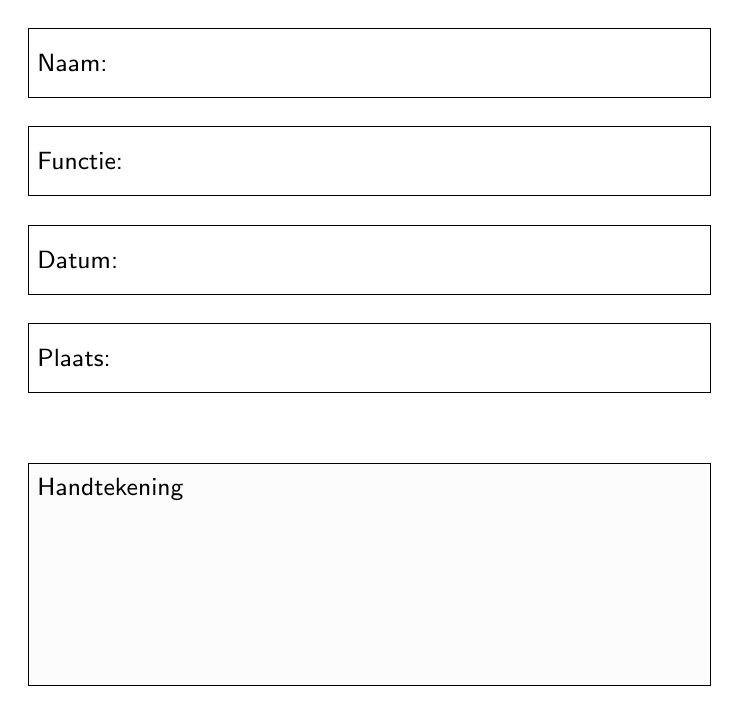
\begin{tikzpicture}
\tikzstyle{every node}=[font=\small];
\node [inputblock] (names) {Naam:};
\node [inputblock, below of = names, node distance = 1.25cm] (function) {Functie:};
\node [inputblock, below of = function, node distance = 1.25cm] (dates) {Datum:};
\node [inputblock, below of = dates, node distance = 1.25cm] (place) {Plaats:};
\node [autographblock, below of = place, node distance = 2.75cm] (autograph) {Handtekening};
\end{tikzpicture}



% table of contents
\renewcommand*\contentsname{Inhoudsopgave}
\tableofcontents

\pagebreak


% The document

% Introductie

\section{Introductie}

\subsection{Management summary}
In het document Technisch Ontwerp \customerdomain \ wordt de technische implementatie beschreven. Het is een blauwdruk voor ontwikkelaars. 

\subsection{Opbouw document}
Dit document dient als leidraad voor de bouw van dit project. Het belangrijkste onderdeel ervan zijn daarom de componenten\seeone{componenten}. Componenten bieden een opsplitsing van de functionaliteiten binnen de website, zowel zichtbaar als niet zichtbaar. Tijdens de bouw zal een ontwikkelaar aan \'{e}\'{e}n specifiek component tegelijk werken. Daarnaast worden in dit document een aantal randzaken zoals deployment\seeone{deployment} en performance\seeone{performance} en algemene eisen\seeone{algemeen} beschreven in eerdere hoofdstukken. In de appendix vindt met een overzicht van Drupal specifieke zaken zoals content types en views, maar ook referentietabellen die aangeven waar welk onderdeel uit het interactieontwerp\seeone{ioto} of de design briefing\seeone{dbto} is beschreven.
\section{Basiselementen, terminologie en definities}

Elk softwaresysteem hanteert bepaald taalgebruik en termen. Dit om een eenduidige betekenis van een term te defini\"eren. Voor het schrijf- en leesgemak van de ontwikkelaars worden dan ook de termen gebruikt die bij Drupal gangbaar zijn. Echter voor een niet-ontwikkelaar of een niet-Drupal gebruiker kan dit verwarring opleveren. 

\begin{description}

\item[Drupal] Drupal is het gekozen Content Management Systeem wat als framework dient voor de bouw van de nieuwe website. Drupal is Open Source CMS welke geschreven is in PHP. 

\item[Modules] Drupal is een modulair gebaseerd systeem. Een module is een verzameling van code welke als uitbreiding dient. In andere systemen wordt dit ook wel een plug-in of extensie genoemd. 

\item[Contrib (contributed) modules] Wanneer gesproken wordt over contrib of contributed modules, wordt hiermee bedoeld de modules die beschikbaar zijn op drupal.org. Dit zijn modules die beschikbaar zijn gesteld door communityleden, welke vrij te verkrijgen zijn. 

\item[Custom modules] Hiermee wordt bedoeld modules die op maat zijn gemaakt omdat de functionaliteit niet beschikbaar is binnen contrib modules. Een custom module kan ook een uitbreiding zijn op een bestaande contrib module. 

\item[Contenttype] Een contenttype is een term die veelgebruikt wordt in Drupal. Het is een type pagina met een zelfde structuur van velden. Een contenttype is bedoeld om onderscheid te kunnen maken tussen het soort inhoud. 

\item[Taxonomy] Voor de categorisering van inhoud wordt gebruik gemaakt van taxonomy. Taxonomy is de term die gebruikt wordt om labels (tags) aan inhoud te koppelen. Dit kunnen vooraf ingestelde lijsten zijn of vrij in te vullen door en voor de gebruiker. 

\item[User] Een gebruiker binnen Drupal.

\item[Roles] Drupal heeft een op rollen gebaseerd permissiesysteem. De rollen zijn configureerbaar en uit te breiden naar wens. 
De standaard rollen die Drupal meelevert zijn:

\item[Anonymous users] Niet-ingelogde gebruikers, bezoekers.
\item[Autenticated users] Ingelogde gebruikers.
\item[Administrator] De rol voor de beheerder van de site. Deze rol mag feitelijk alle pagina's en inhoud bezoeken, alsmede alle instellingen van een website aanpassen. 

\item[Blok] Drupal maakt veel gebruik van blokken (blocks). Een blok is een los element, waar de inhoud van een blok verschillend kan zijn. Een blok kan geplaatst worden op een pagina. Afhankelijk van de implementatie kunnen blokken ook dynamisch getoond worden op basis van context van de pagina. 

\item[Views] Een veelgebruikte contrib module, welke wordt gebruikt om overzichten en lijsten mee te maken (views). Als er gesproken wordt over "een view" dan wordt er verwezen naar een afzonderlijke implementatie van de views module. 

\item[Theme] Een verzameling van bestanden (.PHP, .INFO, .CSS, .JPG, .GIF, .PNG), welke samen het uiterlijk van de website bepalen. Een theme bevat elementen zoals een header, iconen, de indeling van het blokken systeem. 

\item[Template] Een bestand bestaande uit HTML met PHP code, bedoelt om een specifieke structuur te leveren. 

\item[Cache] Drupal genereert (onderdelen van) pagina's en slaat deze op in de cache. Door dit systeem hoeft een pagina niet telkens opnieuw opgebouwd te worden, wat de snelheid ten goede komt. 

\item[CMS] Afkorting: Content Management System, hiermee wordt bedoeld het beheergedeelte van Drupal. 

\item[Core] Het basissysteem en basismodules van Drupal. 

\item[Cron] Een script die gebruikt wordt om automatisch bepaalde zaken uit te voeren. Drupal gebruikt een cronjob om regelmatig terugkerende zaken uit te voeren. 

\item[Entity] Een entity is een verzameling van informatie die niet specifiek inhoudsgebonden is. Een user kan bijvoorbeeld een entity zijn. 

\item[Field] Een field kan een onderdeel zijn van een contenttype of entity. Hiermee kan informatie worden toegevoegd aan een entiteit. 

\item[Menu] Een term die vaak gebruikt wordt om de navigatie mee in te richten. Een menu item is een link in de navigatie. 

\item[Node] Met Node wordt bedoeld een enkel stuk content van een contenttype die door middel van een node-id enkelvoudig wordt beschreven. Een node kan een pagina hebben met een eigen url. 

\item[Region] Een region is een bepaald gedefin\"eerd gedeelte van de website. In een regio kan inhoud worden geplaatst, alsmede blokken.

\end{description}


% Algemeen
\section{Algemeen}\label{algemeen}

\subsection{Webrichtlijnen}

Opgeleverd werk voldoet volledig aan de HTML5 en CSS3 standaard zoals opgesteld door het \emph{World Wide Web consortium}\footnote{http://www.w3.org/standards/webdesign/htmlcss}.

\subsection{Browsers}
Deze paragraaf beschrijft op welke browsers wordt getest bij de bouw. Bij de bouw worden de \emph{best practices} aangehouden waardoor de functionaliteit op meer browsers zal werken dan in dit onderdeel aangegeven.

\subsubsection{Legenda voor desktop browsers en mobile browsers}
In de volgende 2 tabellen worden in de verschillende vakjes, symbolen gebruikt. Deze symbolen hebben een betekenis die in de onderstaande tabel wordt toegelicht.

\begin{tabularx}{\linewidth}{| p{5cm} | X |}
\hline
\rowcolor{tableheader}
\textbf{Symbool} & \textbf{Uitleg} \\ \hline
++	& 100\% stijlen en functionele implementatie \\ \hline
+	& Visueel goed werkend, minimale afwijking   \\ \hline
0	& Functioneel goed werkend, acceptabele      \\ \hline
-	& Strevend functioneel werkend, stijl niet optimaal  \\ \hline
N/A	& Niet van toepassing  \\ \hline
\end{tabularx}

\subsubsection{Desktop browsers}
\begin{tabularx}{\linewidth}{| X | l | l | l | l | l | l l |}
\hline
\rowcolor{tableheader}
��������\textbf{OS}���      & \textbf{IE10} & \textbf{IE9} & \textbf{IE8} & \textbf{Firefox} & \textbf{Chrome} & \textbf{Safari} & \textbf{Opera} \\ \hline
��������Windows 8���������� & ++� & N/A� & N/A & ++����� & ++���� & 0����� & 0���� \\ \hline
��������Windows 7���������� & ++� & ++� & N/A� & ++����� & ++���� & 0����� & 0���� \\ \hline
��������Windows Vista������ & N/A� & ++� & +� & ++����� & ++���� & 0����� & 0���� \\ \hline
��������Windows XP��������� & N/A & N/A & +� & ++����� & 0���� & 0����� & 0���� \\ \hline
��������Windows 2003 Server & N/A & N/A & N/A & ++����� & 0����� & 0����� & 0���� \\ \hline
��������Linux�������������� & N/A� & N/A & N/A & -������ & -��� & -����� & -���� \\ \hline
��������Mac OS������������� & N/A� & N/A & N/A & ++����� & ++���� & ++���� & 0���� \\ \hline
\end{tabularx}

\subsubsection{Mobiele browsers}

\begin{tabularx}{\linewidth}{| X | l | l | l | l | l | l |}
\rowcolor{tableheader}
\hline
��������\textbf{OS}��  & \textbf{Safari} & \textbf{Android} & \textbf{Blackberry} & \textbf{Chrome} & \textbf{Firefox} & \textbf{IEMobile} \\ \hline
��������iOS����������� & ++���� & N/A������������ & N/A������� & +��� & N/A���������� & N/A����� \\ \hline
��������Android������� & N/A��� & ++������������� & N/A������� & +��� & +���������� & N/A����� \\ \hline
��������Blackberry���� & N/A��� & N/A������������ & +�������� & N/A��� & N/A���������� & N/A����� \\ \hline
��������Windows Mobile & N/A��� & N/A������������ & N/A������� & N/A��� & N/A���������� & ++������ \\ \hline
��������Overig�������� & -����� & -�������������� & -��������� & -����� & -������������ & -������� \\ \hline
\end{tabularx}



\subsection{Taal}\label{taal}
De standaardtaal voor Drupal is Engels. De \usemodule{locale} module (uit Drupal core) zal worden ingezet om andere vertalingen te kunnen laten zien. De vertalingen van Drupal zal ge\"{i}mporteerd worden voor de modules waarvoor deze beschikbaar is. De vertalingen kunnen in het beheergedeelte aangevuld c.q. aangepast worden.

Bij oplevering zullen we de volgende talen aanmaken en importeren:
\begin{itemize}
\item Nederlands
\item Engels
\item Duits
\item Frans
\item Italiaans
\end{itemize}

\subsubsection{Datumformaat}
Het standaard datumformaat zullen we instellen op "dd maand yyyy" (bijv. 4 mei 2011).

\subsection{Rechten en rollen}\label{rollen}

zie \emph{Design briefing} vanaf pagina 7.

De volgende rollen worden aangemaakt:
\begin{itemize}
\item eindredacteur
\item redacteur
\end{itemize}

\subsection{Anti-spam}\label{antispam}

Er zullen geen specifieke maatregelen worden getroffen om spam tegen te gaan. 

\subsection{Cookies}\label{cookies}

Om gebruik te mogen maken van Google Analytics en Social Media zal een cookiebalk ingezet worden\seeone{cookiebalk}.

\section{Deployment}\label{deployment}

Voor de deployment (uitrollen van nieuwe releases) en updates van contrib modules maken we gebruik van een \emph{drush make script} en de \usemodule{features} module.

\subsection{Drush make}

Deze techniek is vooral bedoeld om nieuwe Drupal sites op te zetten met \'{e}\'{e}n commando. Grofweg biedt het de volgende mogelijkheden:

\begin{itemize}
  \item Drupal core downloaden
  \item Modules en themes downloaden (zowel contrib als custom via files of versiebeheer)
  \item Patches toepassen
  \item Externe libraries downloaden
\end{itemize}

Drush make zal geen wijzigingen in de database maken en installeert de modules dus niet. Dit kan wel worden gerealiseerd door Drush make te gebruiken in combinatie met andere Drush commando's.

Drush make zal alle bestanden overschrijven wanneer dit op een bestaande installatie wordt gedraaid. Dat maakt het niet onmogelijk om updates via Drush make door te voeren, maar vereist wel een aantal aanpassingen in de werkwijze. Zo moeten alle modules in een eigen repository beheerd worden (svn, git of bzr). Hierbij wordt afgedwongen dat aanpassingen altijd volgens een vaste werkwijze doorgevoerd worden. Aanpassingen in bestaande modules zijn bijvoorbeeld niet mogelijk zonder een werkende patch file mee te leveren. Dat dwingt niet alleen af dat patch files aangemaakt worden, maar ook dat deze aangepast worden in het geval dat de patches met de laatste moduleversies niet meer werken.

De Drupal instantie voor \thecustomer \ zal worden gebouwd met een make script. Dit script houden we bij in de repository. Het makescript is een .sh bestand dat een Drupal core met contrib modules neerzet via \emph{drush make} en daarna de custom modules toevoegt. Het totale resultaat wordt niet in git gezet, maar uitsluitend de makefiles en de custom modules.

De directorystructuur is als volgt:

\begin{itemize}
\item data \\
    Bevat de files directory en (default.)settings.php. Alleen default.settings.php staat in git.
\item modules \\
    Bevat de custom modules.
\item code \\
    Drupal codebase. Staat niet in git, wordt aangemaakt door het make-script
\end{itemize}

De makefiles staan in de repository root.

Voor lokaal gebruik maken we een symlink van de \emph{sites/all/modules/custom} directory naar {modules}. De modules kunnen dan direct in de site aangepast worden terwijl ze toch op de goede plek terecht komen in de repository. Ook de \emph{sites/default} map wordt een symlink (naar \emph{data}) zodat de files en lokale config niet verloren gaan wanneer het make script opnieuw wordt uitgevoerd.

\subsection{Features}

Deze module kan diverse componenten uit de database (bijv. views) exporteren naar een \usemodule{features} module (code). Die module kan vervolgens worden beheerd in SVN of GIT. Dit maakt het uitrollen eenvoudig; door de code bij te werken en de cache te legen wordt alle functionaliteit overgezet. Bij de ontwikkeling kan gewoon de normale workflow worden aangehouden en kunnen contenttypes bijv. met CCK gemaakt worden en views gewoon in de views admin.

Nadeel van deze techniek is dat niet voor alles een integratie met feature bestaat. Er bestaat een integratie tussen features en views, features en CCK, features en context etc. Tegelijkertijd is dat ook de kracht van deze module, want er is ook geen standaard werkwijze mogelijk om elke willekeurige functionaliteit kunnen exporteren en importeren, zonder van de structuur af te weten. De module biedt zelf de volgende integraties aan:

\begin{itemize}
  \item Content types
  \item Velden
  \item Image styles
  \item Menu links
  \item Custom menu's
  \item Permissies
  \item Gebruikersrollen
  \item Taxonomie
  \item Input filters
  \item Views
\end{itemize}

Tevens kunnen afhankelijkheden op andere modules worden aangegeven. Daarmee kan zeker worden gesteld dat nieuwe contrib modules ook meegaan bij de livegang.

Nadeel van features is wel dat features elkaar niet kunnen overlappen. Wanneer bijvoorbeeld twee features afhankelijk zijn van hetzelfde nodetype, dan zal dat nodetype niet in beide features opgenomen kunnen worden. Dit kan verholpen worden door van de overlap een aparte feature module te maken waarvan de oorspronkelijke twee features afhankelijk zijn. Een andere optie is om het nodetype aan \'{e}\'{e}n feature module toe te voegen en een afhankelijkheid op die module toe te voegen aan de andere feature.

\subsection{Release cycle}

Tijdens de bouw (tot aan livegang) wordt alle ontwikkeling in \'{e}\'{e}n branch (\texttt{develop}) gedaan. Dat heeft tot gevolg dat bij een release naar de (pre)prod omgeving \emph{alle} wijzigingen meekomen. Er is dus geen mogelijkheid voor \emph{cherry-picking} (releasen van een specifieke set aan wijzigingen, anders dan alle wijzigingen mee te nemen).
Na de livegang komt er een aparte branch voor de productieomgeving, waardoor \emph{cherry-picking} wel mogelijk is. Vanaf dan moeten we wijzigingen \emph{mergen} voordat deze op productie komen. Tijdens de ontwikkeling wordt dit bewust niet gedaan omdat dit onnodig extra tijd vergt..

Releases naar de verschillende omgevingen worden tijdens de ontwikkeling gedaan wanneer dit noodzakelijk wordt geacht om te testen. Na de livegang zal een vaste releasecycle worden afgesproken (in SLA).



\section{Performance}


\section{Componenten internet}\label{internet}


\subsection{Hoofdnavigatie}

De hoofdnavigatie in de header bestaat uit twee niveau's. De eerste zien eruit als tabbladeren. In de wireframes zijn dit "Inwoners", "Ondernemingen" en "Bestuur". Het tweede niveau zit in de balk daaronder. Het hoofdmenu (tabs + balk eronder) en subnavigatie maken allen gebruik van hetzelfde menu.

\subsection{Topmenu}

Voor het topmenu wordt een apart menu aangemaakt. Hiervoor wordt het standaard menublok uit Drupal core gebruikt.

\subsection{Alfabet}

Het alfabet wordt ingesteld in een blok met custom HTML code. De pagina's daarachter worden gemaakt via \usemodule{views}. Hiervoor wordt een view aangemaakt op het pad \texttt{letter/\%}, waarbij de \% een contextual filter is op nodetitel ("begint met"). De links gaan dus naar \texttt{letter/a}, \texttt{letter/b} etc.

\subsection{Subnavigatie}

De subnavigatie komt in de linkerkolom op pagina's waar dat van toepassing is. Dit blok wordt gebouwd met de \usemodule{submenutree} module. Dit menu begint op het derde niveau en kan t/m het zesde niveau tonen (dus bevat 3 lagen).

\subsection{Footer}

De footer bestaat uit 3 kolommen en is vrij in te vullen door de redactie. Hiervoor worden 3 Felix regio's aangemaakt\seeone{felix}. De inhoud van de footer is voor elke pagina van de subsite gelijk.



\subsection{Zoeken}\label{zoeken}

Voor \drupalpath wordt de \emph{Solr module} gebruikt, deze module vervangt de standaard \emph{Drupal Search module}. 
De \emph{Solr module} biedt naast de standaard zoek functionaliteit ook meer geavanceerde functionaliteiten zoals zoeken in bijlagen, markeren van zoekwoorden en de mogelijkheid tot het aanpassen van de \emph{Bias settings}. 

\subsubsection{Bias settings}

\emph{Bias settings} maken het mogelijk inhoud voorrang te geven in de zoekresultaten. Je kunt bijvoorbeeld het inhoudstype \emph{Nieuws} meer punten geven dan het inhoudstype \emph{Bekendmaking}. Hoe hoger het aantal toegekende punten hoe meer voorrang het krijgt. 

Ga naar \drupalpath{admin/config/search/apachesolr} en klik vervolgens op \emph{Bias} bij de betreffende website om de \emph{Bias settings} aan te passen. Let op: het is niet aangeraden om zonder voldoende kennis deze settings aan te passen.

\begin{center}
	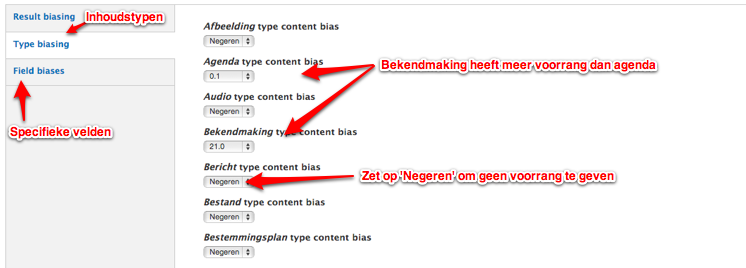
\includegraphics[width=\textwidth]{img/bias.png}
\end{center}

Klik na het bewerken op de knop \emph{Instellingen opslaan} om de \emph{Bias settings} op te slaan. 

\subsubsection{Content uitsluiten van zoekmachine}

Het is mogelijk om specifieke nodes uit te sluiten van indexatie in de interne zoekmachine. Klik onderaan het bewerkformulier op het tabblad \emph{Uitsluiten uit zoekresultaten} en vink de checkbox aan, zie onderataand afbeelding.

\begin{center}
	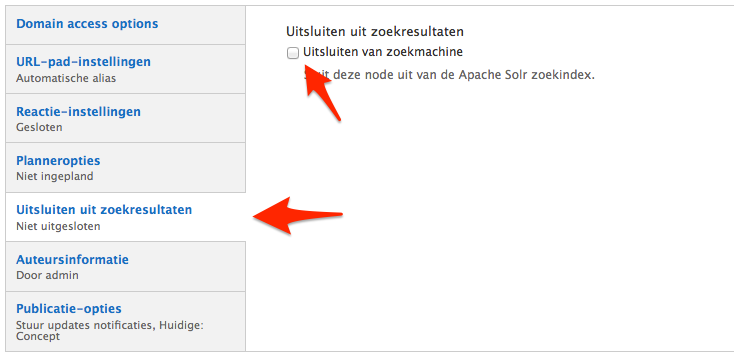
\includegraphics[width=\textwidth]{img/solr-exclude.png}
\end{center}

\subsubsection{Synoniemen beheren}

Solr biedt ondersteuning voor synoniemen. Hiermee kan worden ingesteld dat een zoekopdracht naar "i-pad" ook inhoud met de tekst "ipad" wordt opgenomen in de resultaten.

De synoniemen zijn te beheren via Drupal. Ga hiervoor naar \\ \drupalpath{admin/config/search/apachesolr/synonyms}. Op deze pagina is een lijst te vinden met de huidige synoniemen. Deze kunnen hier worden aangepast of uit de lijst worden gehaald. Onder de lijst is een formulier zichtbaar waarmee nieuwe synoniemen toegevoegd kunnen worden. Het trefwoord is het originele woord (bijv. "ipad") en de synoniemen worden ingevoerd als een komma gescheiden lijst (bijv. "i-pad, i pad").

Nieuwe synoniemen treden niet direct in werking. De lijst wordt iedere nacht doorgezet naar de Solr server. In dit proces wordt tevens de ingestelde lijst samengevoegd met de basislijst (generieke lijst voor alle gemeentes).

\subsection{Tekstpagina}\label{tekstpagina}

Voor de tekstpagina's wordt het standaard nodetype \texttt{page} gebruikt.

Het is mogelijk om in de tekst afbeeldingen op te nemen via de media bibliotheek\seeone{media}. Onder de bodytekst kunnen blokken worden toegevoegd voor bijv. een carrousel\seeone{felix}.

\subsubsection{Inline tabs}

Op tekstpagina's moet het mogelijk zijn om inline tabs op te nemen. In plaats van \'{e}\'{e}n stuk tekst wordt de indeling dan als volgt:
\begin{verbatim}
[introtekst]
[tabs]
[tekst van actieve tab]
\end{verbatim}
Het actieve tab is altijd de eerste, totdat een ander tabblad wordt aangeklikt. Het aantal tabs is ongelimiteerd. Wel kan er maar \'{e}\'{e}n set tabs per pagina worden gebruikt.
De invoer van de tabs gebeurt in het body veld. Elke heading die begint met "**" wordt omgezet naar een tab. De volgende invoer:
\begin{verbatim}
<p>Introtekst</p>
<h2>Titel</h2>
<p>Meer tekst...</p>
<h2>**Eerste</h2>
<p>Tekst in eerste tabblad</p>
<h2>**Tweede</h2>
<p>Tekst in tweede tabblad</p>
<p>Meer tekst in tweede tabblad</p>
\end{verbatim}
wordt omgezet naar:
\begin{verbatim}
<p>Introtekst</p>
<h2>Titel</h2>
<p>Meer tekst...</p>
<div class="inlinetabs">
  <ul>
    <li><a href="#inlinetabs-[id]"><span>Eerste</span></a></li>
    <li><a href="#inlinetabs-[id]"><span>Tweede</span></a></li>
  </ul>
  <div id="inlinetabs-[id]">
    <p>Tekst in eerste tabblad</p>
  </div>
  <div id="inlinetabs-[id]">
    <p>Tekst in tweede tabblad</p>
    <p>Meer tekst in tweede tabblad</p>
  </div>
</div>
\end{verbatim}
De tekst \texttt{[id]} is een unieke code voor dat tabblad en wordt random gegenereerd. De omzetting vind plaats in een input filter en wordt ge\"{i}mplementeerd in een custom module met de naam \texttt{inlinetabs}. Hierin wordt ook een JavaScript toegevoegd om de tabs actief te maken middels jQuery UI Tabs\footnote{http://api.jqueryui.com/tabs/}.

Het nieuwe input filter zetten we aan op \emph{filtered html} en \emph{full html}. Dit filter wordt aan het eind toegevoegd om te voorkomen dat de id's en classes verdwijnen.

\subsubsection{404 en 403 pagina's}\label{404pagina}

De 404 en 403 pagina's zijn een speciaal soort tekstpagina.

Om te voorkomen dat deze pagina's in de zoekresultaten komt doen we een aanpassing in de \texttt{bespoke} module zodat deze niet meegenomen wordt in het zoekresultaat (via de \texttt{apachesolr\_query\_alter}-hook).

Deze pagina is niet geiljk aan de storingspagina voor fouten uit de \texttt{5xx}-categorie\seeone{storingspagina}.


\subsection{Agenda \& Evenementen}\label{agenda-en-evenementen}

\subsubsection{Overzicht}\label{agendaoverzicht}

De overzichtspagina van de agenda is een lijstpagina met alle projecten die beginnen vanaf vandaag, gesorteerd op begindatum. In de rechter zijbalk wordt een blok toegevoegd met langlopende evenementen. Dit zijn evenementen die eerder dan vandaag zijn begonnen, maar nog steeds bezig zijn.

\subsubsection{Agenda detailpagina}\label{agenda-detail}

Een agenda item bevat de volgende velden die op de node detailpagina worden getoond:
\begin{itemize}
\item Titel
\item Datum (inclusief tot-datum indien beschikbaar)
\item Tijd
\item Toegang
\item Locatie
\item Afbeelding
\item Body tekst
\end{itemize}
Alleen de tekstuele locatie wordt getoond (indien beschikbaar). De co\"{o}rdinaten zijn wel in te voeren. De hier beschreven velden zijn de velden die op de detailpagina worden getoond, dus niet de referentie van beschikbare velden\seeone{sec:content-event}.

In de sidebar aan de rechterkant worden eveneens enkele velden ontsloten m.b.v. de \usemodule{cck\_blocks} module:
\begin{itemize}
\item Formulieren (nodereference),
\item Externe links (link field).
\end{itemize}

\subsubsection{Agenda teaser blok}

View die een teaser view laten zien van de laatste drie items van type Agenda, gesorteerd op aanmaakdatum. Zie \seeref{laatste-agenda-items}

Teaser view bevat:
\begin{itemize}
\item Titel,
\item Datum (optioneel met tot-datum)
\item en "Lees meer" link naar node detailpagina.
\end{itemize}
\subsection{Nieuws}\label{nieuws}

\subsubsection{Laatste nieuws}

Via felix wordt het mogelijk om de view te tonen met de laatste drie nieuwsitems. Zie \seeref{laatste-nieuws-items}

\subsubsection{Nieuwsarchief}

Een view met een overzicht van alle nieuwsitems. Zie \seeref{nieuws-overzicht}.

\subsubsection{Nieuws detailpagina}

Is gelijk aan detailpagina van standaardpagina.
\subsection{Bekendmakingen}\label{bekendmakingen}

Bekendmakingen worden opgeslagen als Drupal nodes. Deze worden ge\"{i}mporteerd uit GVOP.

\subsubsection{Kaart en lijstweergave}\label{bekendmakingen-op-de-kaart}

De kaart wordt ontwikkeld m.b.v. views. Zie \seeref{bekendmakingen-markers}. De tekstuele resultaten worden middels een attachment bij deze view ingeladen \seeref{bekendmakingen-overzicht}.

De kaart wordt gemaakt met de \usemodule{gmap} module i.c.m. \usemodule{views}. Via \emph{exposed filters} wordt de volgende filtering aangeboden (in een apart blok):
\begin{itemize}
\item Zoeken op titel
\item Datum (van / tot)
\item Postcode (alleen exacte matching)
\item Status aanvraag (taxonomie, via checkboxes)
\end{itemize}
De filtering heeft zowel invloed op de kaart als op de lijst onder de kaart.


\subsection{Poll}

Voor de poll wordt de \texttt{poll} module uit Drupal core ingezet.
Elke poll heeft een aparte pagina (detailpagina), maar het is ook mogelijk om de poll in andere pagina's op te nemen middels de \usemodule{felix} module als redactioneel blok\seeone{felix}.

De poll heeft enkel een multiple choise optie, met \'{e}\'{e}n vraag per poll.

\subsection{Redactionele blokken}\label{felix}

De module \usemodule{felix} wordt ingezet om het voor redacteuren mogelijk te maken om redactionele blokken te plaatsen binnen vooraf gedefinieerde regio's. Welke regio's dat zijn wordt in deze sectie verder uitgewerkt. Alle blokken die worden geplaatst zijn specifiek voor \'{e}\'{e}n pagina en worden dus niet automatisch op meerdere (gerelateerde) pagina's geplaatst. De blokken zijn wel generiek over alle subsites. Wanneer een blok op \texttt{/nieuws} wordt geplaatst dan zal deze op een andere subsite ook zichtbaar zijn op dat pad, mits de geplaatste node ook op dat domein is gepubliceerd.

Onderstaand tabel geeft een overzicht van de Felix regio's.

\begin{tabularx}{\linewidth}{| p{3cm} | p{3cm} | X | p{3cm} | }
\hline
\rowcolor{tableheader}
\textbf{Naam} & \textbf{Systeemnaam} & \textbf{Verschillend per} & \textbf{Positie} \\ \hline
Paginaspecifiek & sidebar\_path & path & rechter zijbalk \\ \hline
Paginatype & sidebar\_node & nodetype & rechter zijbalk \\ \hline
Inhoud & content & path & onder de content \\ \hline
Footer kolom 1 & footer1 & domain & footer \\ \hline
Footer kolom 2 & footer2 & domain & footer \\ \hline
Footer kolom 3 & footer3 & domain & footer \\ \hline
\end{tabularx}

Om de blokken te kunnen scheiden per domein wordt gebruik gemaakt van de \usemodule{felix\_domain} submodule. In de rechterkolom worden twee regio's gebruikt. Blokken die geplaatst worden in de ene regio zijn specifiek voor die pagina. De andere regio is verschillend per nodetype. Als daarin een blok wordt geplaatst op een bekendmaking detailpagina dan zal deze op alle detailpagina's van bekendmakingen te zien zijn. De volgorde van de blokken kan alleen worden aangepast binnen de regio. Blokken die specifiek zijn voor de pagina staan altijd onder de blokken die generiek zijn voor het nodetype. Hierop wordt het gewicht van de regio's aangepast.

Er wordt \'{e}\'{e}n \emph{blockset} aangemaakt. De blokken die vrij te plaatsen zijn kunnen dus in elke regio worden gezet. De theming is wel afhankelijk van de regio (wordt volledig in CSS geregeld). In de rest van dit onderdeel wordt aangegeven welke blokken er mogelijk zijn, met screenshots.

\subsubsection{Blokken per content type}\label{felixcontenttypeblokken}

Voor alle nodetypes die een detailpagina hebben wordt een blok aangemaakt met links naar de laatste 5 gepubliceerde items. Dit blok kan binnen elke felix regio redactioneel worden ingesteld.


\subsection{Social media}

Ter ondersteuning van het delen op social media wordt voorzien in de volgende zaken:
\begin{itemize}
\item Share buttons
\item Mogelijkheid om widgets in HTML code te plaatsen
\item RSS feeds
\end{itemize}

\subsubsection{Share buttons}

De share buttons geven de mogelijkheid om de pagina te delen op de verschillende sociale media. Hierin kunnen de volgende buttons worden ingesteld:
\begin{itemize}
\item Facebook
\item Google+
\item LinkedIn
\item Twitter
\item Delen op Facebook (widget)
\item Twitteren (widget)
\end{itemize}

Bij oplevering van de standaarddistributie worden de specifieke share links aangezet. De widgets worden niet ingesteld. Deze kunnen bij implementatie van de gemeentesites makkelijk worden aangezet. De theming zal wel geschikt worden gemaakt voor het grotere formaat van deze widgets.

Buttons worden op alle nodetypes toegevoegd die een detailpagina hebben.

Per subsite wordt instelbaar of de share buttons direct zichtbaar zijn of onder een overlay komen. In het laatste geval is een enkele "delen" link beschikbaar waarmee de overlay geopend kan worden. Voor deze instelling wordt een custom \emph{dominion functie} aangemaakt met de systeemnaam \texttt{sharelink}. In het theme kan dan gebruik gemaakt worden van de functie \texttt{dominion\_has\_function} om te bepalen of de overlay gebruikt moet worden.

\subsubsection{Widgets in HTML-code}

Eindredacteuren krijgen de mogelijkheid om zelf HTML widgets te plaatsen in de body tekst\seeone{invoerformaten}.

\subsubsection{Externe RSS-feeds}

Via de \usemodule{views} module i.c.m. de \usemodule{views\_rss} module worden RSS feeds ingesteld. De volgende feeds worden aangemaakt:
\begin{enumerate}
\item Laatste nieuwsberichten
\item Actuele evenementen
\item Laatste bekendmakingen
\item Laatst gewijzigde pagina's
\end{enumerate}
De views worden gesorteerd op publicatiedatum (1 t/m 3) of datum laatst gewijzigd (4). De RSS feed laat altijd 20 items zien.

Nieuwe RSS feeds kunnen niet door de gemeente aangemaakt worden.


\subsection{Forum}\label{forum}
Te vinden op \drupalpath{forum}.

\subsubsection{Aanmaken forumcategorieen}\label{forumcategorieen}
Op \drupalpath{admin/structure/taxonomy/forums} zijn forumonderwerpen aan te maken. Dit zijn de onderwerpen op het hoogste niveau binnen het forum. Voor de onderwerpen worden taxonomietermen gebruik.

\subsubsection{Aanmaken forumonderwerpen}\label{forumonderwerpen}
Het aanmaken van een nieuw forumonderwerp doe je door op de knop \emph{Forumonderwerp toevoegen} te drukken. Hierna volgt een itembewerkpagina waar je het onderwerp kan aanmaken. Selecteer een forumcategorie (Forums) om het onderwerp in een van de categorieen te plaatsen. Maak je een nieuw onderwerp aan binnen een categorie zal deze automatisch geselecteerd zijn.

\begin{center}
	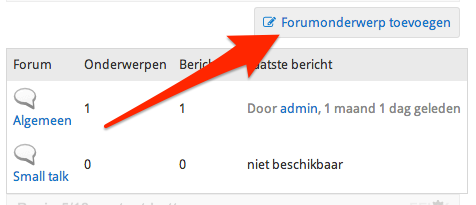
\includegraphics[width=\textwidth]{img/forumonderwerp.png}
\end{center}
\subsection{Multisite}\label{multisite}

Voor de ondersteuning van subsites (waaronder ook het intranet) wordt de \usemodule{dominion} module ingezet. Hiermee kan een eindredacteur zelf nieuwe sites aanmaken.

\subsubsection{Algemene dominion config}
Voor de \usemodule{dominion} module worden de volgende settings aangepast:
\begin{itemize}
\item Default host suffix: .gemeente.nl (later per gemeente in te stellen)
\item Editor roles: redacteurrol aanvinkens
\end{itemize}

\subsubsection{Subsite menu}
Onder de instellingen van \usemodule{dominion\_menu} wordt een domein specifiek menu ingesteld. Het bijbehorende menublok wordt ingesteld in de linkerkolom.

\subsubsection{Zoeken en multisite}
De \texttt{dominion\_apachesolr} module wordt gebruikt om ervoor te zorgen dat zoekopdrachten alleen resultaten teruggeven van de huidige subsite. Indien wenselijk kan wel per subsite worden aangegeven of er nog additionele domein mee worden genomen. De zoekresultaten komen in dat geval door elkaar. Deze optie wordt ook gebruikt om automatisch onderliggende domeinen mee te nemen, zoals de team subsites op het intranet.

\subsubsection{Views}
Alle views die nodes laten zien worden aangepast. Er wordt een extra filter toegevoegd dat alleen nodes laat zien die op het huidige domein zijn gepubliceerd ("Domain: Available on current domain"). Dit om te voorkomen dat gebruikers met de "bypass node access" permissie content van alle domeinen in de views te zien krijgen.

\subsubsection{Permissies}
De domain module biedt de mogelijkheid om gebruikers aan domeinen te koppelen. Dit systeem staat los van de gebruikersrollen die gebruikers hebben. Een aantal permissies heeft alleen effect wanneer de gebruiker ook aan het domein is gekoppeld (bijvoorbeeld het aanmaken van nieuwe inhoud). De gebruiker heeft dus deze rechten wanneer  hij / zij \'{e}n de juiste gebruikersrol heeft, \'{e}n gekoppeld is aan het domein. Dat wil tevens zeggen dat een gebruiker niet een redacteur kan zijn op het ene domein en een eindredacteur op het andere domein. In een later stadium kan eventueel een module gemaakt worden waarmee het wel mogelijk is om verschillende rollen toe te wijzen per gebruiker / domein combinatie.

\subsubsection{Functionaliteit}
Per subsite kan aangevinkt worden welke functionaliteit beschikbaar is. De volgende opties zijn beschikbaar:
\begin{itemize}
\item Nieuws
\item Agenda
\item Contactformulier
\end{itemize}
Dit is geen uitputtende lijst van functionaliteiten, maar bevat enkel de opties die aan- of uitgezet kunnen worden. Bijvoorbeeld een tekstpagina is altijd beschikbaar.
\subsection{Wysiwyg en media}\label{wysiwyg}

Voor media en wysiwyg worden de \usemodule{wysiwyg} en \usemodule{media} / \usemodule{file\_entity} modules ingezet. Als editor zelf wordt gekozen voor \texttt{CKEditor} aangezien dit de meestgebruikte editor is binnen Drupal en standaard is in Drupal 8.

\subsubsection{Buttons}

De buttons staan gespecificeerd in het FO document.
Een aantal buttons zit niet standaard in de \usemodule{wysiwyg} module. Hiervoor wordt de reeds ontwikkelde \texttt{ckeditor\_customtags} module gebruikt waarmee buttons kunnen worden toegevoegd.

\subsubsection{Links in bodytekst}

Voor het gemakkelijk kunnen toevoegen van links in bodyteksten wordt gebruik gemaakt van de \usemodule{linkit} module i.c.m. \usemodule{pathologic}.

\subsubsection{Invoerformaten}\label{invoerformaten}

Er worden drie invoerformaten ter beschikking gesteld voor gebruikers en redacteuren.

\begin{itemize}
\item \textbf{Full HTML} \\
Volledige HTML zonder filtering. Alleen beschikbaar voor eindredacteuren. Het wordt aanbevolen om hier spaarzaam gebruik van te maken vanwege de mogelijkheid om nieuwe XSS issues (security issues) te introduceren.
\item \textbf{Filtered HTML} \\
Standaard filtering op ongewenste HTML en herschrijven van links door \texttt{pathologic}.
\item \textbf{Plain text} \\
Wordt gebruikt voor reviews (geplaatst door bezoekers). Hierbij wordt geen opmaak / HTML toegestaan.
\end{itemize}

\subsubsection{Media}\label{media}

Images en video's moeten toegevoegd en hergebruikt kunnen worden in wysiwyg en bestandsvelden.
Uitgangspunt is versie 2 van de \texttt{media} module.



\subsection{Hansel}

De module \usemodule{hansel} is oorspronkelijk gemaakt om flexibel de breadcrumbs aan te kunnen passen. Hansel kan (en zal) ingezet worden voor de volgende functionaliteiten:
\begin{itemize}
\item Breadcrumbs
\item Vriendelijke URL-paden
\item Activeren van menu-items
\end{itemize}

\subsection{Google Analytics}\label{analytics}

We zullen de standaard \usemodule{googleanalytics} module inzetten. Hierbij gaan we uit van basis tracking. Er worden dus geen aanvullende tellers of rapportages ingesteld. \thecustomer \ zal het Google Analytics account aanmaken en de accountcode aanleveren.
\subsection{Sitemap}\label{sitemap}
De sitemap wordt standaard ingesteld tijdens de installatie van Dimpact. Mocht je de sitemap toch naar wens willen aanpassen dan kun je dit doen via de volgende link: \drupalpath{admin/config/search/sitemap}

In dit formulier kun je aangeven wat er in de sitemap moet komen te staan. Voer bij \emph{Paginatitel} een titel voor de pagina in. Onder \emph{Sitemap bericht} kan je een tekst plaatsen die op de pagina zichtbaar is. 

Onder \emph{SITEMAP INHOUD} kan je kiezen voor de volgende instellingen. \emph{Geef de voorpagina weer}, plaats een link naar de voorpagina. \emph{Menu's die in de sitemap moeten worden opgenomen}, geef aan welke menu's getoond moeten worden als lijstweergave op de sitemap. \emph{Geef FAQ inhoud weer}, toont een lijst met FAQ items. \emph{Categorieen die in de sitemap moeten worden opgenomen}, toont een lijst met taxonomietermen die binnen de vocabulaires vallen.

Onder \emph{CATEGORIE-INSTELLINGEN} stel je de weergavemodus in voor de te tonen taxonomietermen. \emph{Show node counts by categories} toont het aantal gekoppelde nodes aan een taxonomieterm. \emph{Categories depth} geef de diepte op tot op welk niveau termen opgehaald moeten worden. \emph{thresholds} geven aan vanaf hoeveel gekoppelde items de term weergegeven moet worden.

Onder \emph{RSS-INSTELLINGEN} stel je de instellingen in voor de RSS feed. Onder \emph{CSS SETTINGS} kan je opgeven of je het CSS bestand bij de RSS feed wilt inladen.

Klik onderaan de pagina op de knop \emph{Instellingen opslaan} om te instellingen op te slaan. De sitemap wordt dan beschikbaar op /sitemap.
\subsection{Nieuwsbrieven}\label{nieuwsbrieven}

Voor het versturen van nieuwsbrieven wordt gebruik gemaakt van \emph{MailChimp}. Voor de integratie wordt gebruik gemaakt van de \usemodule{mailchimp} module. Iedere gemeente maakt gebruik van zijn eigen MailChimp account. In het MailChimp account moet een API-key worden aangemaakt op:
\begin{verbatim}
https://admin.mailchimp.com/account/api/
\end{verbatim}
Deze key wordt ingesteld in de settings van de \usemodule{mailchimp} module. Naast de basismodule worden ook de \texttt{mailchimp\_campaign} en \texttt{mailchimp\_lists} modules aangezet. Met de laatste module kunnen mailing lists ook in Drupal worden aangemaakt. Daardoor komt een blok beschikbaar waarmee bezoekers zich kunnen aanmelden voor de mailinglist. Bij het aanmaken van de lijst in Drupal worden de volgende settings gebruikt:
\begin{itemize}
\item Label: naam van de mailinglist (gelijk aan de naam in MailChimp)
\item MailChimp list: lijst zoals aangemaakt in MailChimp
\item Allow anonymous registrations: aangevinkt
\item Roles: allen
\item List label: naam van de mailinglist (gelijk aan de naam in MailChimp)
\end{itemize}
Het blok voor de mailinglist wordt ingesteld in \usemodule{felix}.
\subsection{Storingspagina}\label{storingspagina}

Er wordt een storingspagina ontworpen. Zowel de Drupal "offline" page en de Varnish foutpagina worden hierop aangepast. Deze pagina is niet binnen Drupal te beheren.

\subsection{Cookiebalk}\label{cookiebalk}
De instellingen van deze module zijn te vinden op: \drupalpath{admin/config/user-interface/cookie-consent}. De volgende instellingen kunnen worden aangepast:

\begin{itemize}
\item \emph{More information Node Link}. Vul hier de titel van de node in waar de informatie over het cookiegebruik van de website op staat.
\item \emph{More information Link Title}. Vul hier de tekst van de meer informatie-knop in.
\item \emph{Rolen}. De rollen die de cookiebalk te zien krijgen.
\item \emph{Exclude Cookie Consent}. Vul hier de paden van pagina's in waarop de cookiebalk niet te zien mag zijn.
\item \emph{Exclude Domains}. Selecteer domeinen waarop de cookiebalk niet te zien mag zijn.
\item \emph{Cookie Consent Style}. Bepaal het uiterlijk van de balk. Dit kan licht, donker of monochrome (zwart/wit) zijn.
\item \emph{Hide the privacy tab}. Verberg het tabblad.
\item \emph{Privacy Tab Position}. Plaats van het tabblad op in het browserscherm.
\item \emph{Banner position}. De positie van de cookiebalk.
\item \emph{Refresh on consent}. Ververs de pagina wanneer de gebruiker akkoord heeft gegeven op het gebruik van cookies. 
\item \emph{Filter iframe tags}. Toon geen inhoud van iframes zolang er geen akkoord is gegeven op het gebruik van cookies.
\item \emph{Stricly necessary Scripts}, \emph{Social Media Scripts}, \emph{Advertising Scripts}, \emph{Analytics Scripts}. Hier kunnen scripts worden opgevoerd die uitgevoerd moeten worden na akkoord.
\end{itemize}
\subsection{Readspeaker}\label{readspeaker}

Voor de voorleesfunctie zullen we gebruikmaken van ReadSpeaker. De integratie hiervan gebeurt in het theme. Per gemeente wordt een apart account aangemaakt. Bij ReadSpeaker dienen hiervoor de relevante domeinen te worden ingesteld waarop deze actief wordt. De \emph{customer id} is nodig in Drupal.

In \texttt{page.tpl.php} wordt de volgende code gebruikt op de plaats waar de button moet komen:

\begin{lstlisting}[language=PHP]
  <?php $readspeaker_customerid = variable_get('readspeaker_customerid', 0); ?>
  <?php if ($readspeaker_customerid): ?>
  <div id="readspeaker_button1" class="rs_skip rsbtn rs_preserve">
    <a class="rsbtn_play" title="Laat de tekst voorlezen met ReadSpeaker" href="//app.eu.readspeaker.com/cgi-bin/rsent?customerid=<?php print $readspeaker_customerid; ?>&amp;lang=nl_nl&amp;readid=main&amp;url=<?php echo urlencode($_SERVER['HTTP_HOST'] . $_SERVER['REQUEST_URI']); ?>">
        <span class="rsbtn_left rsimg rspart"><span class="rsbtn_text"><span>Lees voor</span></span></span>
        <span class="rsbtn_right rsimg rsplay rspart"></span>
    </a>
  </div>
  <?php endif; ?>
\end{lstlisting}

In \texttt{html.tpl.php} wordt de volgende code gezet binnen de \texttt{\textless head\textgreater}:
\begin{lstlisting}[language=PHP]
<script src="<?php print base_path() . path_to_theme() . '/readspeaker/ReadSpeaker.js?pids=embhl'; ?>"></script>
\end{lstlisting}

De JavaScripts van readspeaker worden zelf gehost en dus ook in het theme gezet. Dat is nodig om de button te laten werken op SSL.

De \emph{customer id} kan worden ingesteld in \texttt{settings.php}:
\begin{lstlisting}[language=PHP]
$conf['readspeaker_customerid] = 1234;
\end{lstlisting}

Wanneer deze niet gezet is zal de button niet worden getoond.
\subsection{Dashboard}\label{dashboard}
Het dashboard is de persoonlijke pagina voor ieder lid van het Intranet. Het is een pagina die is opgebouwd uit blokken die de gebruiker zelf kan aanzetten, uitzetten of verplaatsen.

In de onderstaande afbeelding zie je het Dashboard voor een Intranet gebruiker. 
Bij pijl 1 kun je blokken toevoegen aan je Dashboard. Elk blok heeft verschillende opties zoals inklappen, uitklappen en sluiten. Deze zijn te vinden bij pijl 2

\begin{center}
	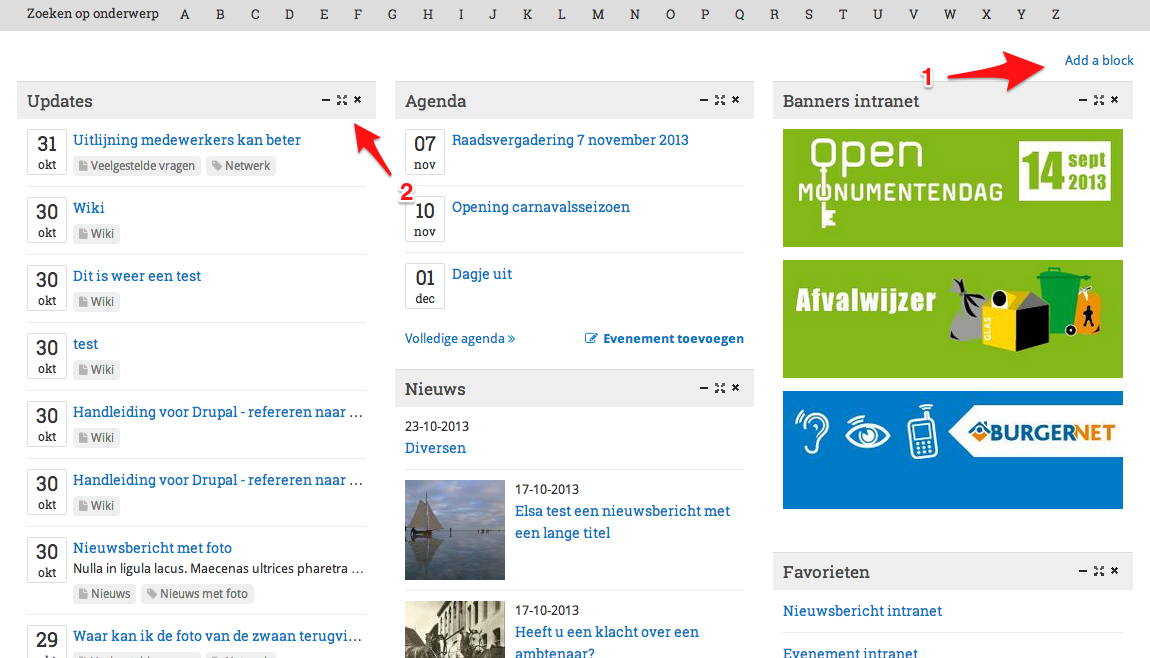
\includegraphics[width=\textwidth]{img/dashboard.png}
\end{center}
\subsection{SSL}

Voor de formulieren zal gebruik worden gemaakt van SSL. Dit moet zo worden ingericht dat:
\begin{itemize}
\item bezoekers automatisch op https terecht komen wanneer ze op de webshop terecht komen of inloggen
\item session cookies niet over http verstuurd worden
\item bezoekers automatisch op https terecht komen wanneer ze ingelogd zijn (op https) en ze bezoeken een pagina over http.
\end{itemize}
 De encryptie wordt op een SSL offloader (bijv. \emph{Pound}) ingericht welke het verkeer doorstuurd naar Varnish. Bij het doorsturen van dit verkeer wordt een header meegestuurd waardoor Varnish en Drupal kunnen herkennen dat het verkeer oorspronkelijk vanaf https afkomstig is. Dat is nodig om te bepalen of de bezoeker wel of niet doorgestuurd moet worden naar een andere versie. Hiervoor wordt de \texttt{X-Forwarded-Proto} header gebruikt met als waarde \texttt{https}. Andere headers zijn mogelijk, maar dit is de de facto standaard.

In Drupal wordt de \texttt{settings.php} aangepast. Ten eerste wordt de \emph{mixed mode} uitgezet. Daardoor zijn sessies over https niet bruikbaar over http. De setting \texttt{session.cookie\_secure} wordt aangepast om ervoor te zorgen dat session cookies niet verstuurd worden over http. Dat zou namelijk een security lek opleveren omdat de session token dan alsnog lekt wanneer men per ongeluk op http komt (door bijv. het gebruik van links in mail of bookmarks).

\begin{lstlisting}[language=PHP]
$conf['https'] = FALSE;
ini_set('session.cookie_secure', 1);
\end{lstlisting}

Daarnaast wordt de SSL modus 'aangezet' wanneer de \texttt{X-Forwarded-Proto} header is gevonden en de waarde "https" heeft.

\begin{lstlisting}[language=PHP]
if (isset($_SERVER['HTTP_X_FORWARDED_PROTO']) && strtolower($_SERVER['HTTP_X_FORWARDED_PROTO']) == 'https') {
  $_SERVER['HTTPS'] = 'on';
}
\end{lstlisting}

In de \texttt{bespoke} module wordt code toegevoegd om een \texttt{ssl} cookie te zetten wanneer men op ssl zit. Deze wordt gebruikt om bezoekers op http te redirecten naar https indien ze daar mogelijk ingelogd zijn. Of ze daar werkelijk ingelogd zijn valt in dat stadium niet te achterhalen, omdat de session token alleen meegestuurd wordt over https (vanwege de \emph{secure} flag). De code in \texttt{bespoke} is als volgt:

\begin{lstlisting}[language=PHP]
function bespoke_init() {
  global $is_https;
  if ($is_https && empty($_COOKIE['ssl'])) {
    // Set a marker to know that the user is logged in via SSL.
    $params = session_get_cookie_params();
    $expire = $params['lifetime'] ? REQUEST_TIME + $params['lifetime'] : 0;
    setcookie('ssl', 1, $expire, $params['path'], $params['domain'], FALSE, TRUE);
  }
}
\end{lstlisting}

De redirect zelf wordt gedaan in de \texttt{settings.php}:

\begin{lstlisting}[language=PHP]
if (!empty($_COOKIE['ssl']) && empty($_SERVER['HTTPS'])) {
  header('Location: https://' . $_SERVER['HTTP_HOST'] . $_SERVER['REQUEST_URI'], TRUE, 302);
  exit;
}
\end{lstlisting}

Merk op dat de \texttt{ssl} cookie invloed heeft op het wel of niet kunnen cachen in Varnish. De cookie wordt daarom niet gefilterd in de \texttt{vcl\_recv} functie\seeone{varnishrecv}.

In de \texttt{bespoke} module wordt de html code van iedere pagina aangepast om ervoor te zorgen dat links binnen \texttt{https} blijven wanneer men over SSL de site bezoekt en vice-versa. De canonical URL vormt hierop een uitzondering. Daar wordt altijd de \texttt{http} versie gebruikt, omdat anders de \texttt{http} en \texttt{https} versies beide ge\"{i}ndexeerd kunnen worden waardoor \emph{duplicate content} ontstaat. Voor de implementatie hiervan wordt \texttt{hook\_page\_alter} gebruikt waarin een functie wordt toegevoegd aan \texttt{\$page['\#post\_render']}. In die functie wordt de HTML via find \& replace aangepast op basis van de global variable \texttt{\$is\_https}.

Als laatste wordt de \usemodule{securepages} module ingezet om ervoor te zorgen dat bezoekers automatisch op https terecht komen wanneer ze inloggen.

\subsection{Mobile variant}\label{mobile}

De website wordt responsive opgezet. Uitzondering is de homepage waar tevens een adaptive variant beschikbaar is voor mobiele telefoons. De detectie hiervan vindt plaats in Varnish\seeone{varnishmobile}. De aanpassing in Varnish zorgt ervoor dat de pagina op \texttt{/voorpagina-mobiel} wordt geladen wanneer de voorpagina wordt bezocht met een mobiele telefoon. Hierbij wordt geen redirect gebruikt. Het pad is voor de bezoeker dan ook niet zichtbaar. De pagina kan ook op de desktop worden geladen door direct dit pad te gebruiken. Dat zal worden gedaan om de inhoud van de pagina te kunnen bewerken ("beheermodus").

In het theme zullen we zorgen dat een ander page template wordt gebruikt voor de mobiele homepage. Hiervoor zullen we een aanpassing doen in de \texttt{hook\_preprocess\_page}. Belangrijk is dat de canonical url hierbij niet \texttt{voorpagina-mobiel} is maar de echte voorpagina. Daarom zullen we de volgende code gebruiken:

\begin{lstlisting}[language=HTML]
<link rel="canonical" href="http://<?php print check_plain($_SERVER['HTTP_HOST']); ?>/" />
\end{lstlisting}

\subsection{Unit Tests}

Zorg er bij elke test voor dat de configuratie, modules en permissies goed worden ge�nstalleerd. Zorg er eveneens voor dat een Unit Test bestaat uit besloten functionaliteit. Vuistregel: indien een test meer dan 1 ding doet, is het waarschijnlijk beter om hiervoor twee losse Unit tests te schrijven met een dependency.

Het schrijven van de test:
\begin{itemize}
\item \texttt{getInfo}. Deze method geeft de naam, beschrijving en de groep waar deze unit test deel van uitmaakt.
\item \texttt{setUp}. Deze method definieert dependencies die nodig zijn om de tests succesvol te kunnen draaien. Denk aan het aanzetten van modules die noodzakelijk zijn, het aanmaken en inloggen van de testgebruiker, permissies etc.
\item \texttt{testSimpleTextX}. Deze method bevat de test zelf. Schrijf hierin duidelijk op (in comments) wat de test behoort te doen, en zorg ervoor dat aan alle condities wordt voldaan.
\end{itemize}

Om de noodzakelijke configuratie voor de Unit Tests gemakkelijker te kunnen beheren, wordt er een feature gemaakt waarin alle dependencies worden opgenomen. Het aanzetten van deze feature dient te resulteren in een complete installatie van het \projectname  project.




\section{Componenten intranet}\label{intranet}

\subsection{LDAP}\label{ldap}

Login gaat via LDAP of Active Directory (protocol compatible). Hiervoor wordt de \usemodule{ldap} module ingezet. Deze module voorziet in het importeren van gegevens uit LDAP in het Drupal profiel. Het gaat hier om de naam en functie. Aangezien LDAP op verschillende manieren ingezet kan worden zullen de precieze velden met de gemeente afgestemd moeten worden bij de gemeente specifieke implementatie.

\subsection{Google Analytics}\label{analytics}

We zullen de standaard \usemodule{googleanalytics} module inzetten. Hierbij gaan we uit van basis tracking. Er worden dus geen aanvullende tellers of rapportages ingesteld. \thecustomer \ zal het Google Analytics account aanmaken en de accountcode aanleveren.
\subsection{Dashboard}\label{dashboard}
Het dashboard is de persoonlijke pagina voor ieder lid van het Intranet. Het is een pagina die is opgebouwd uit blokken die de gebruiker zelf kan aanzetten, uitzetten of verplaatsen.

In de onderstaande afbeelding zie je het Dashboard voor een Intranet gebruiker. 
Bij pijl 1 kun je blokken toevoegen aan je Dashboard. Elk blok heeft verschillende opties zoals inklappen, uitklappen en sluiten. Deze zijn te vinden bij pijl 2

\begin{center}
	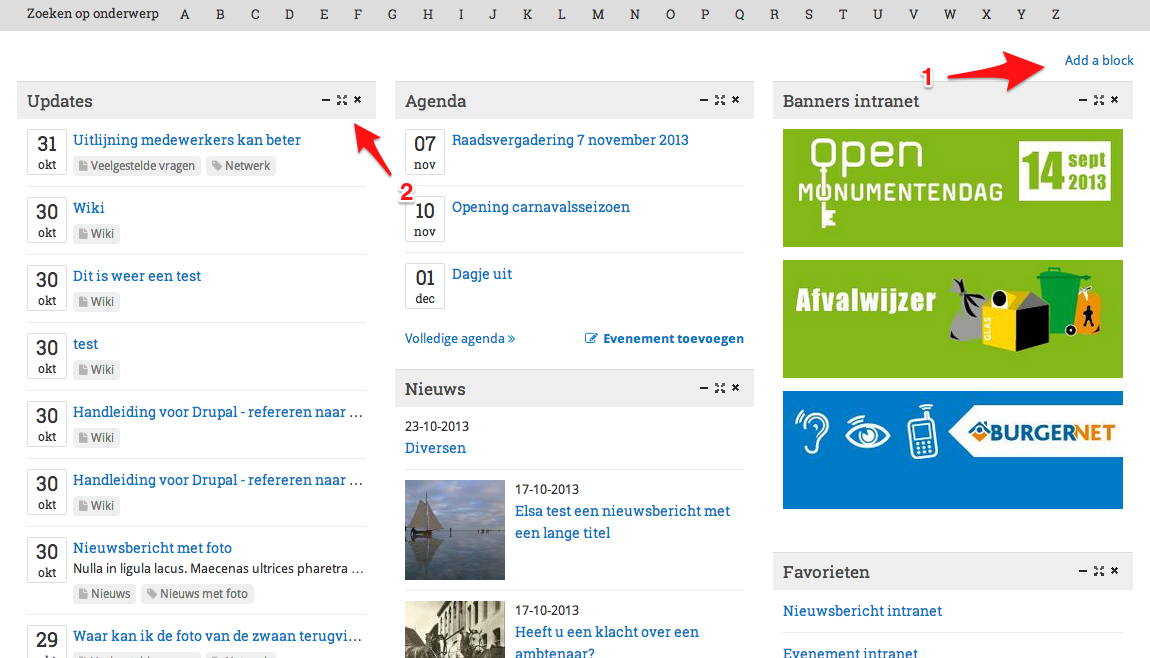
\includegraphics[width=\textwidth]{img/dashboard.png}
\end{center}
\subsection{Smoelenboek}
\label{sec:smoelenboek}

\begin{itemize}
  \item Tabsblok met nieuws en agenda zie \ref{sec:tabsmetnieuwsenagenda}
  \item Grafisch element blok zie \ref{sec:grafischelement}
\end{itemize}
\subsection{Wie is online}\label{wieisonline}

In Drupal core zit een blok "Who's online". Dit blok gebruiken we echter niet direct aangezien hier ook burgers tussen zullen zitten. In een custom module met de naam \texttt{dimpact\_whoisonline} wordt de code hiervan gekopieerd en aangepast zodat alleen users met de rol "medewerker" in deze lijst voorkomen.

\subsection{Persoonlijk profiel}\label{profiel}

In het persoonlijk staan de volgende elementen:
\begin{itemize}
\item Foto
\item Algemene gegevens
\item Vrije tekstvelden
\begin{itemize}
\item Persoonlijke gegevens
\item Kennis/opleidingen/werk
\item Activiteiten/interesses
\item Overige informatie
\end{itemize}
\item Mijn projecten
\item Mijn producten
\item Mijn foto's
\item Links en downloads
\end{itemize}
De algemene gegevens zijn vooraf ingevuld en niet aanpasbaar.
Voor het aanpassen van de gegevens wordt gebruik gemaakt van de \usemodule{profile2} module i.c.m. de submodule \usemodule{profile2\_pages}. Hierin worden de volgende profielen aangemaakt:
\begin{itemize}
\item Profielfoto \\ Bevat een enkel filefield om een profielfoto te kunnen uploaden.
\\ Systeemnaam: \texttt{avatar}
\item Persoonlijk profiel \\ Bevat de vier vrije tekstvelden
\\ Systeemnaam: \texttt{personal}
\item Mijn projecten \\ Bevat een link veld (multiple) waarin gebruikers zelf links kunnen plaatsen.
\\ Systeemnaam: \texttt{projects}
\item Mijn producten \\ Bevat een link veld (multiple) waarin gebruikers zelf links kunnen plaatsen.
\\ Systeemnaam: \texttt{products}
\item Mijn foto's \\ Bevat een media veld (multiple)
\\ Systeemnaam: \texttt{photos}
\item Links en downloads \\ Bevat een link veld (multiple) waarin gebruikers zelf links kunnen plaatsen.
\\ Systeemnaam: \texttt{links}
\end{itemize}
Elk profiel type heeft een eigen pagina waarop de inhoud kan worden bewerkt. Deze pagina is beschikbaar op \texttt{profile-[name]/[uid]/edit}, waarbij \texttt{[name]} de systeemnaam is en \texttt{[uid]} de \emph{user id}. Wanneer men op het eigen profiel op \emph{Bewerken} klinkt dan komt men op \texttt{profile-personal/[uid]/edit}.

De \usemodule{profile2} module heeft een integratie met de \usemodule{views} module. Voor alle profiel types behalve persoonlijke informatie worden via de views module blokken gemaakt. Hierbij wordt de user id uit de URL gehaald via een contextual filter. In de footer van de view wordt via PHP code een link naar de bewerkpagina getoond indien het user id uit de url overeenkomt met de user id van de bezoeker.

De profielinformatie wat via de beschreven pagina's wordt aangepast blijft binnen Drupal en wordt niet verzonden naar andere systemen (zoals LDAP).
\subsection{Favorieten}\label{favorieten}

Via de \usemodule{views} en \usemodule{flag} module wordt het voor medewerkers mogelijk om pagina's als "favoriet" aan te merken. De lijst van favorieten is vervolgens terug te vinden op het dashboard\seeone{dashboard}. Er wordt een nieuw flag type aangemaakt met de volgende settings:
\begin{itemize}
\item Title: "Favoriet" (machine name: "favorite")
\item Flag link text: "Toevoegen als favoriet"
\item Unflag link text: "Verwijderen uit favorieten"
\item Flag access: medewerker- en redacteurrollen
\item Bundles: agenda, basic page, blog, wiki
\item Display link as field: aanvinken
\end{itemize}
Voor alle overige settings wordt de standaardinstelling gebruikt. Met de laatste setting wordt een link toegevoegd aan de detailpagina's die in de favorieten kunnen worden gezet.


\subsection{Marktplaats}\label{marktplaats}

Op de marktplaats krijgen gebruikers van het intranet de mogelijkheid om berichten te plaatsen waar anderen op kunnen reageren. Nieuwe items worden automatisch gepubliceerd. Gebruikers kunnen hun eigen berichten aanpassen en verwijderen.

\subsection{Nieuwsfeeds}\label{nieuwsfeeds}

Via de \usemodule{feeds} module wordt een vaste set aan nieuwsfeeds ge\"{i}mporteerd. Per feed is een blok beschikbaar dat kan worden ingesteld in het dashboard\seeone{dashboard}. Voor dit blok wordt de \usemodule{views} module gebruikt.

\subsection{Wiki}\label{wiki}

Voor de wiki functionaliteit zullen we gebruikmaken van de \usemodule{wikitools} module. Tevens wordt een nieuw nodetype aangemaakt voor wikipagina's. Dit nodetype is gelijk aan een standaardpagina. Het pad (via \usemodule{pathauto}) is echter "wiki/[node:title]". Voor wikitools worden de volgende settings aangepast:
\begin{itemize}
\item Titel van voorpagina: Wiki
\item Node types: wiki
\item Wiki 404 type: Creation form
\end{itemize}
Voor alle overige settings worden de standaardwaarden gebruikt. De wiki is dan beschikbaar op \texttt{/wiki}. We zullen de voorpagina tijdens de bouw aanmaken.

In de bodytekst van wiki nodes kunnen links worden gebruikt naar \texttt{/wiki/Titel\_van\_pagina} (spaties dienen vervangen te worden door underscores). Bij het bezoeken van niet bestaande pagina's is een link beschikbaar om die pagina direct aan te maken.

Er wordt een custom module gemaakt welke een input filter aanbiedt waarmee makkelijk links naar wiki pagina's kunnen worden gemaakt. Dit wordt uitgewerkt in een module met de naam \texttt{wiki\_links}.

Tekst voor filtering:
\begin{verbatim}
[[Titel van pagina]]
[[Titel van pagina|Titel van link]]
\end{verbatim}
Tekst na filtering:
\begin{verbatim}
<a href="/wiki/Titel_van_pagina">Titel van pagina</a>
<a href="/wiki/Titel_van_pagina">Titel van link</a>
\end{verbatim}
In het pad worden spaties vervangen door underscores.

De \texttt{freelinking} module biedt vrijwel identieke functionaliteit aan, maar werkt niet voor pagina's die niet bestaan en is daarom voor een wiki minder goed bruikbaar.


\subsection{Blog}\label{blog}

Via de \usemodule{views} maken we een overzicht van alle blog nodes per user. Een voorbeeld van een blog pagina is peter/blog. Een algemeen overzicht van alle aanwezige blog is te vinden op /blog. 
\subsection{Foto-album}\label{fotoalbum}



\subsection{Notificaties}\label{notificaties}

Gebruikers van het intranet (lees: medewerkers) moeten de mogelijkheid krijgen om zich te abonneren op nieuwe inhoud en wijzigingen van inhoud. Hiervoor wordt de \usemodule{subscriptions} module gebruikt (inclusief de dependency \usemodule{mail\_edit}). De volgende settings worden aangepast:
\begin{itemize}
\item Unlisted content types: editorial, slide
\item Node form position: Fieldset in Subscriptions interface block
\item Node form visibility: Display only a Subscribe link that makes the fieldset visible 
\item Expand the node form fieldset: aangevinkt
\item E-mail address: gelijk aan site\_mail (via code in settings.php)
\item Display watchdog entries for successful mailings: uitgevinkt (vanwege performance)
\end{itemize}
Het blok \emph{Subscriptions interface} wordt aangezet in de content region.
De tekst in de mail wordt via de \usemodule{mail\_edit} module vertaald naar Nederlands.

In de \texttt{bespoke} module passen we via \texttt{alter}-functies de pagina met de subscribe opties aan (\texttt{node/\%/subscribe}). Op deze pagina staat het formulier waarmee de gebruiker zich kan abonneren. De node content daarboven halen we weg. Ook zetten we de opties niet langer in een fieldset, waardoor de link "Subscribe" op deze pagina zal verdwijnen.


\subsection{Teampagina}\label{teampagina}

De teampagina is een verzamelpunt van agenda items, berichten, veelgestelde vragen en documenten van een specifiek team. Hiervoor wordt gebruik gemaakt van subsites via \usemodule{dominion}. De subsites worden op een directory geplaatst, bijv. \texttt{/teams/communicatie}. De directory is tevens het pad van de teampagina, dat feitelijk de homepage is van de subsite. Toevoegen van inhoud moet ook vanaf de subsite, op bijv. \texttt{team/communicatie/node/add/event}.

\subsubsection{Blokken}

De landingspagina (voorpagina) van de team subsite wordt gemaakt met de \usemodule{emptypage} module. Deze is bij het aanmaken volledig blanco. Ook de rechterkolom is leeg. Via \usemodule{felix}\seeone{felix} kunnen de volgende blokken worden geplaatst:
\begin{itemize}
\item Laatste 5 agenda items
\item Laatste 5 berichten
\item Laatste 5 veelgestelde vragen
\item Laatste 5 documenten
\end{itemize}
De bedoeling is dat ieder team deze blokken naar eigen inzicht kan verdelen over de middenkolom en de rechterkolom.

De blokken worden gemaakt met \usemodule{views}. Om de theming hiervan onafhankelijk te maken van de blokken met laatste 5 nodes van het internet\seeone{felixcontenttypeblokken} wordt hiervoor een nieuwe view gemaakt. In de footer worden links naar de \texttt{node/add/\%} pagina's getoond indien de bezoeker daar toegang toe heeft. Dit moet gecontroleerd worden via de \texttt{dominion\_restrict} module:

\begin{verbatim}
global $user;
if (dominion_restrict_node_access('event', 'create', $user) {
  print l(t('Evenement toevoegen'), 'node/add/event');
}
\end{verbatim}

De lees meer link gaat naar een lijstweergave van alle items.

\subsubsection{Medewerkers lijst}

Onderaan de landingspagina wordt een lijst van medewerkers getoond. Deze lijst wordt gemaakt met de \usemodule{views} module. Dit is een lijst van profielen via \usemodule{profile2} module\seeone{profiel} van gebruikers die gekoppeld zijn aan het huidige domein.


\clearpage

\appendix
\appendixpage\label{appendices}
\addappheadtotoc

\section{Content Types}
\subsection{Agenda}
\label{sec:content-agenda}
Reacties zijn bij items van dit content type standaard uitgeschakeld, maar wel zichtbaar (dit is per item aan te passen).

\subsubsection{Velden}
  \begin{longtable}{| p{3.75cm}|p{3.75cm}|p{7.50cm}|}
  \hline
  \rowcolor{tableheader}
  \textbf{Veld} & \textbf{Type} & \textbf{Omschrijving}  \tabularnewline
  \hline
\endfirsthead
\multicolumn{3}{l}{\textit{Vervolg van vorige pagina}} \\
\hline
\rowcolor{tableheader}
  \textbf{Veld} & \textbf{Type} & \textbf{Omschrijving}  \tabularnewline
  \hline
\hline
\endhead
\multicolumn{3}{r}{\textit{Gaat verder op volgende pagina}} \\
\endfoot
\hline
\endlastfoot
  \raggedright{Title} & \raggedright{Tekst} & \raggedright{}  \tabularnewline
  \hline
  \raggedright{Intro} & \raggedright{Tekst} & \raggedright{}  \tabularnewline
  \hline
  \raggedright{Body} & \raggedright{WYSIWYG (met samenvatting)} & \raggedright{}  \tabularnewline
  \hline
  \raggedright{Image} & \raggedright{Bestand} & \raggedright{}  \tabularnewline
  \hline
  \raggedright{Date} & \raggedright{Datum} & \raggedright{}  \tabularnewline
  \hline
  \raggedright{Time} & \raggedright{Datum} & \raggedright{}  \tabularnewline
  \hline
  \raggedright{Location} & \raggedright{location} & \raggedright{}  \tabularnewline
  \hline
  \raggedright{Add to calendar} & \raggedright{Datum} & \raggedright{Choose a date to publish the node to the calender.}  \tabularnewline
  \hline
  \end{longtable}

\subsection{Announcement}
\label{sec:content-announcement}
Reacties zijn bij items van dit content type standaard uitgeschakeld, maar wel zichtbaar (dit is per item aan te passen).

\subsubsection{Velden}
  \begin{longtable}{| p{3.75cm}|p{3.75cm}|p{7.50cm}|}
  \hline
  \rowcolor{tableheader}
  \textbf{Veld} & \textbf{Type} & \textbf{Omschrijving}  \tabularnewline
  \hline
\endfirsthead
\multicolumn{3}{l}{\textit{Vervolg van vorige pagina}} \\
\hline
\rowcolor{tableheader}
  \textbf{Veld} & \textbf{Type} & \textbf{Omschrijving}  \tabularnewline
  \hline
\hline
\endhead
\multicolumn{3}{r}{\textit{Gaat verder op volgende pagina}} \\
\endfoot
\hline
\endlastfoot
  \raggedright{Title} & \raggedright{Tekst} & \raggedright{}  \tabularnewline
  \hline
  \raggedright{Body} & \raggedright{WYSIWYG (met samenvatting)} & \raggedright{}  \tabularnewline
  \hline
  \raggedright{Location} & \raggedright{location} & \raggedright{}  \tabularnewline
  \hline
  \raggedright{Add to calendar} & \raggedright{Datum} & \raggedright{}  \tabularnewline
  \hline
  \end{longtable}

\subsection{Basic page}
\label{sec:content-basic page}
Reacties zijn bij items van dit content type standaard uitgeschakeld, maar wel zichtbaar (dit is per item aan te passen).

\subsubsection{Velden}
  \begin{longtable}{| p{3.75cm}|p{3.75cm}|p{7.50cm}|}
  \hline
  \rowcolor{tableheader}
  \textbf{Veld} & \textbf{Type} & \textbf{Omschrijving}  \tabularnewline
  \hline
\endfirsthead
\multicolumn{3}{l}{\textit{Vervolg van vorige pagina}} \\
\hline
\rowcolor{tableheader}
  \textbf{Veld} & \textbf{Type} & \textbf{Omschrijving}  \tabularnewline
  \hline
\hline
\endhead
\multicolumn{3}{r}{\textit{Gaat verder op volgende pagina}} \\
\endfoot
\hline
\endlastfoot
  \raggedright{Title} & \raggedright{Tekst} & \raggedright{}  \tabularnewline
  \hline
  \raggedright{Body} & \raggedright{WYSIWYG (met samenvatting)} & \raggedright{}  \tabularnewline
  \hline
  \raggedright{Location} & \raggedright{location} & \raggedright{}  \tabularnewline
  \hline
  \raggedright{Add to calendar} & \raggedright{Datum} & \raggedright{}  \tabularnewline
  \hline
  \end{longtable}

\subsection{Blog}
\label{sec:content-blog}
Reacties zijn bij items van dit content type standaard uitgeschakeld (dit is per item aan te passen).

\subsubsection{Velden}
  \begin{longtable}{| p{3.75cm}|p{3.75cm}|p{7.50cm}|}
  \hline
  \rowcolor{tableheader}
  \textbf{Veld} & \textbf{Type} & \textbf{Omschrijving}  \tabularnewline
  \hline
\endfirsthead
\multicolumn{3}{l}{\textit{Vervolg van vorige pagina}} \\
\hline
\rowcolor{tableheader}
  \textbf{Veld} & \textbf{Type} & \textbf{Omschrijving}  \tabularnewline
  \hline
\hline
\endhead
\multicolumn{3}{r}{\textit{Gaat verder op volgende pagina}} \\
\endfoot
\hline
\endlastfoot
  \raggedright{Title} & \raggedright{Tekst} & \raggedright{}  \tabularnewline
  \hline
  \raggedright{Intro} & \raggedright{Tekst} & \raggedright{}  \tabularnewline
  \hline
  \raggedright{Body} & \raggedright{WYSIWYG (met samenvatting)} & \raggedright{}  \tabularnewline
  \hline
  \raggedright{Tags} & \raggedright{Taxonomie (autocomplete)} & \raggedright{}  \tabularnewline
  \hline
  \end{longtable}

\subsection{Editorial}
\label{sec:content-editorial}
Reacties zijn bij items van dit content type standaard uitgeschakeld, maar wel zichtbaar (dit is per item aan te passen).

\subsubsection{Velden}
  \begin{longtable}{| p{3.75cm}|p{3.75cm}|p{7.50cm}|}
  \hline
  \rowcolor{tableheader}
  \textbf{Veld} & \textbf{Type} & \textbf{Omschrijving}  \tabularnewline
  \hline
\endfirsthead
\multicolumn{3}{l}{\textit{Vervolg van vorige pagina}} \\
\hline
\rowcolor{tableheader}
  \textbf{Veld} & \textbf{Type} & \textbf{Omschrijving}  \tabularnewline
  \hline
\hline
\endhead
\multicolumn{3}{r}{\textit{Gaat verder op volgende pagina}} \\
\endfoot
\hline
\endlastfoot
  \raggedright{Title} & \raggedright{Tekst} & \raggedright{}  \tabularnewline
  \hline
  \raggedright{Body} & \raggedright{WYSIWYG (met samenvatting)} & \raggedright{}  \tabularnewline
  \hline
  \end{longtable}

\subsection{FAQ}
\label{sec:content-faq}
Reacties zijn bij items van dit content type standaard uitgeschakeld, maar wel zichtbaar (dit is per item aan te passen).

\subsubsection{Velden}
  \begin{longtable}{| p{3.75cm}|p{3.75cm}|p{7.50cm}|}
  \hline
  \rowcolor{tableheader}
  \textbf{Veld} & \textbf{Type} & \textbf{Omschrijving}  \tabularnewline
  \hline
\endfirsthead
\multicolumn{3}{l}{\textit{Vervolg van vorige pagina}} \\
\hline
\rowcolor{tableheader}
  \textbf{Veld} & \textbf{Type} & \textbf{Omschrijving}  \tabularnewline
  \hline
\hline
\endhead
\multicolumn{3}{r}{\textit{Gaat verder op volgende pagina}} \\
\endfoot
\hline
\endlastfoot
  \raggedright{Title} & \raggedright{Tekst} & \raggedright{}  \tabularnewline
  \hline
  \raggedright{Body} & \raggedright{WYSIWYG (met samenvatting)} & \raggedright{}  \tabularnewline
  \hline
  \raggedright{Location} & \raggedright{location} & \raggedright{}  \tabularnewline
  \hline
  \end{longtable}

\subsection{Marketplace}
\label{sec:content-marketplace}
Reacties zijn bij items van dit content type standaard uitgeschakeld (dit is per item aan te passen).

\subsubsection{Velden}
  \begin{longtable}{| p{3.75cm}|p{3.75cm}|p{7.50cm}|}
  \hline
  \rowcolor{tableheader}
  \textbf{Veld} & \textbf{Type} & \textbf{Omschrijving}  \tabularnewline
  \hline
\endfirsthead
\multicolumn{3}{l}{\textit{Vervolg van vorige pagina}} \\
\hline
\rowcolor{tableheader}
  \textbf{Veld} & \textbf{Type} & \textbf{Omschrijving}  \tabularnewline
  \hline
\hline
\endhead
\multicolumn{3}{r}{\textit{Gaat verder op volgende pagina}} \\
\endfoot
\hline
\endlastfoot
  \raggedright{Title} & \raggedright{Tekst} & \raggedright{}  \tabularnewline
  \hline
  \raggedright{Body} & \raggedright{WYSIWYG (met samenvatting)} & \raggedright{}  \tabularnewline
  \hline
  \raggedright{Category} & \raggedright{Taxonomie (dropdown)} & \raggedright{}  \tabularnewline
  \hline
  \end{longtable}

\subsection{News}
\label{sec:content-news}
Reacties zijn bij items van dit content type standaard uitgeschakeld, maar wel zichtbaar (dit is per item aan te passen).

\subsubsection{Velden}
  \begin{longtable}{| p{3.75cm}|p{3.75cm}|p{7.50cm}|}
  \hline
  \rowcolor{tableheader}
  \textbf{Veld} & \textbf{Type} & \textbf{Omschrijving}  \tabularnewline
  \hline
\endfirsthead
\multicolumn{3}{l}{\textit{Vervolg van vorige pagina}} \\
\hline
\rowcolor{tableheader}
  \textbf{Veld} & \textbf{Type} & \textbf{Omschrijving}  \tabularnewline
  \hline
\hline
\endhead
\multicolumn{3}{r}{\textit{Gaat verder op volgende pagina}} \\
\endfoot
\hline
\endlastfoot
  \raggedright{Title} & \raggedright{Tekst} & \raggedright{}  \tabularnewline
  \hline
  \raggedright{Intro} & \raggedright{Tekst} & \raggedright{}  \tabularnewline
  \hline
  \raggedright{Body} & \raggedright{WYSIWYG (met samenvatting)} & \raggedright{}  \tabularnewline
  \hline
  \raggedright{Image} & \raggedright{Bestand} & \raggedright{}  \tabularnewline
  \hline
  \raggedright{Tags} & \raggedright{Taxonomie (autocomplete)} & \raggedright{}  \tabularnewline
  \hline
  \raggedright{Location} & \raggedright{location} & \raggedright{}  \tabularnewline
  \hline
  \raggedright{Add to calendar} & \raggedright{Datum} & \raggedright{}  \tabularnewline
  \hline
  \end{longtable}

\subsection{Person}
\label{sec:content-person}
Reacties zijn bij items van dit content type standaard uitgeschakeld (dit is per item aan te passen).

\subsubsection{Velden}
  \begin{longtable}{| p{3.75cm}|p{3.75cm}|p{7.50cm}|}
  \hline
  \rowcolor{tableheader}
  \textbf{Veld} & \textbf{Type} & \textbf{Omschrijving}  \tabularnewline
  \hline
\endfirsthead
\multicolumn{3}{l}{\textit{Vervolg van vorige pagina}} \\
\hline
\rowcolor{tableheader}
  \textbf{Veld} & \textbf{Type} & \textbf{Omschrijving}  \tabularnewline
  \hline
\hline
\endhead
\multicolumn{3}{r}{\textit{Gaat verder op volgende pagina}} \\
\endfoot
\hline
\endlastfoot
  \raggedright{Title} & \raggedright{Tekst} & \raggedright{}  \tabularnewline
  \hline
  \raggedright{Image} & \raggedright{Bestand} & \raggedright{}  \tabularnewline
  \hline
  \raggedright{Category} & \raggedright{Radio-knoppen/vinkjes} & \raggedright{}  \tabularnewline
  \hline
  \raggedright{Body} & \raggedright{WYSIWYG (met samenvatting)} & \raggedright{}  \tabularnewline
  \hline
  \end{longtable}

\subsection{Poll}
\label{sec:content-poll}
A poll is a question with a set of possible responses. A poll, once created, automatically provides a simple running count of the number of votes received for each response.

Reacties zijn bij items van dit content type standaard uitgeschakeld (dit is per item aan te passen).

\subsubsection{Velden}
  \begin{longtable}{| p{3.75cm}|p{3.75cm}|p{7.50cm}|}
  \hline
  \rowcolor{tableheader}
  \textbf{Veld} & \textbf{Type} & \textbf{Omschrijving}  \tabularnewline
  \hline
\endfirsthead
\multicolumn{3}{l}{\textit{Vervolg van vorige pagina}} \\
\hline
\rowcolor{tableheader}
  \textbf{Veld} & \textbf{Type} & \textbf{Omschrijving}  \tabularnewline
  \hline
\hline
\endhead
\multicolumn{3}{r}{\textit{Gaat verder op volgende pagina}} \\
\endfoot
\hline
\endlastfoot
  \raggedright{Question} & \raggedright{Tekst} & \raggedright{}  \tabularnewline
  \hline
  \raggedright{Location} & \raggedright{location} & \raggedright{}  \tabularnewline
  \hline
  \end{longtable}

\subsection{Product}
\label{sec:content-product}
Reacties zijn bij items van dit content type standaard uitgeschakeld, maar wel zichtbaar (dit is per item aan te passen).

\subsubsection{Velden}
  \begin{longtable}{| p{3.75cm}|p{3.75cm}|p{7.50cm}|}
  \hline
  \rowcolor{tableheader}
  \textbf{Veld} & \textbf{Type} & \textbf{Omschrijving}  \tabularnewline
  \hline
\endfirsthead
\multicolumn{3}{l}{\textit{Vervolg van vorige pagina}} \\
\hline
\rowcolor{tableheader}
  \textbf{Veld} & \textbf{Type} & \textbf{Omschrijving}  \tabularnewline
  \hline
\hline
\endhead
\multicolumn{3}{r}{\textit{Gaat verder op volgende pagina}} \\
\endfoot
\hline
\endlastfoot
  \raggedright{Title} & \raggedright{Tekst} & \raggedright{}  \tabularnewline
  \hline
  \raggedright{Body} & \raggedright{WYSIWYG (met samenvatting)} & \raggedright{}  \tabularnewline
  \hline
  \raggedright{Location} & \raggedright{location} & \raggedright{}  \tabularnewline
  \hline
  \end{longtable}

\subsection{Slide}
\label{sec:content-slide}
Reacties zijn bij items van dit content type standaard uitgeschakeld, maar wel zichtbaar (dit is per item aan te passen).

\subsubsection{Velden}
  \begin{longtable}{| p{3.75cm}|p{3.75cm}|p{7.50cm}|}
  \hline
  \rowcolor{tableheader}
  \textbf{Veld} & \textbf{Type} & \textbf{Omschrijving}  \tabularnewline
  \hline
\endfirsthead
\multicolumn{3}{l}{\textit{Vervolg van vorige pagina}} \\
\hline
\rowcolor{tableheader}
  \textbf{Veld} & \textbf{Type} & \textbf{Omschrijving}  \tabularnewline
  \hline
\hline
\endhead
\multicolumn{3}{r}{\textit{Gaat verder op volgende pagina}} \\
\endfoot
\hline
\endlastfoot
  \raggedright{Title} & \raggedright{Tekst} & \raggedright{}  \tabularnewline
  \hline
  \raggedright{Body} & \raggedright{WYSIWYG (met samenvatting)} & \raggedright{}  \tabularnewline
  \hline
  \raggedright{Image} & \raggedright{Bestand} & \raggedright{}  \tabularnewline
  \hline
  \end{longtable}

\subsection{Webform}
\label{sec:content-webform}
Create a new form or questionnaire accessible to users. Submission results and statistics are recorded and accessible to privileged users.

Reacties zijn bij items van dit content type standaard uitgeschakeld (dit is per item aan te passen).

\subsubsection{Velden}
  \begin{longtable}{| p{3.75cm}|p{3.75cm}|p{7.50cm}|}
  \hline
  \rowcolor{tableheader}
  \textbf{Veld} & \textbf{Type} & \textbf{Omschrijving}  \tabularnewline
  \hline
\endfirsthead
\multicolumn{3}{l}{\textit{Vervolg van vorige pagina}} \\
\hline
\rowcolor{tableheader}
  \textbf{Veld} & \textbf{Type} & \textbf{Omschrijving}  \tabularnewline
  \hline
\hline
\endhead
\multicolumn{3}{r}{\textit{Gaat verder op volgende pagina}} \\
\endfoot
\hline
\endlastfoot
  \raggedright{Title} & \raggedright{Tekst} & \raggedright{}  \tabularnewline
  \hline
  \raggedright{Body} & \raggedright{WYSIWYG (met samenvatting)} & \raggedright{}  \tabularnewline
  \hline
  \raggedright{Location} & \raggedright{location} & \raggedright{}  \tabularnewline
  \hline
  \raggedright{Add to calendar} & \raggedright{Datum} & \raggedright{}  \tabularnewline
  \hline
  \end{longtable}

\subsection{Wiki}
\label{sec:content-wiki}
Reacties zijn bij items van dit content type standaard uitgeschakeld (dit is per item aan te passen).

\subsubsection{Velden}
  \begin{longtable}{| p{3.75cm}|p{3.75cm}|p{7.50cm}|}
  \hline
  \rowcolor{tableheader}
  \textbf{Veld} & \textbf{Type} & \textbf{Omschrijving}  \tabularnewline
  \hline
\endfirsthead
\multicolumn{3}{l}{\textit{Vervolg van vorige pagina}} \\
\hline
\rowcolor{tableheader}
  \textbf{Veld} & \textbf{Type} & \textbf{Omschrijving}  \tabularnewline
  \hline
\hline
\endhead
\multicolumn{3}{r}{\textit{Gaat verder op volgende pagina}} \\
\endfoot
\hline
\endlastfoot
  \raggedright{Title} & \raggedright{Tekst} & \raggedright{}  \tabularnewline
  \hline
  \raggedright{Body} & \raggedright{WYSIWYG (met samenvatting)} & \raggedright{}  \tabularnewline
  \hline
  \end{longtable}


\subsection{Taxonomie}\label{taxonomie}

Taxonomie wordt gebruikt voor lijsten van woorden. Bijvoorbeeld: de lijst �FAQ categorie�n� bevat de woorden 'Netwerk' en 'Werkplekken'. Taxonomie lijsten kunnen altijd aangepast worden.

\bigskip

\begin{center}
	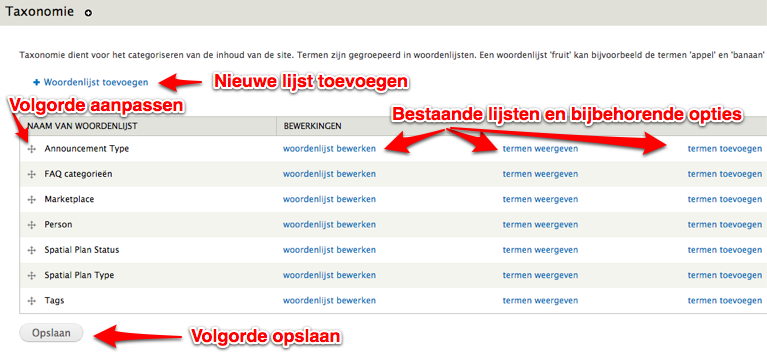
\includegraphics[width=\textwidth]{img/taxonomie2.png}
\end{center}

\subsubsection{Woorden aan woordenlijsten toevoegen}

Ga naar het overzicht van alle woordenlijsten. Klik op 'Termen toevoegen' bij de lijst waaraan je woorden wil toevoegen. Vul bij het veld 'Naam' het woord in en vul eventueel een beschrijving in. Klik onderaan de pagina op de knop 'Opslaan' om het woord aan de lijst toe te voegen. Herhaal deze stappen om meerdere woorden toe te voegen aan de woordenlijst. 

\subsubsection{Woorden in woordenlijsten bewerken}

Het is mogelijk om specifieke woorden uit lijsten te bewerken. Klik op 'Termen weergeven' bij de betreffende lijst.
Klik op 'Bewerken' bij het betreffende woord, vervolgens kun je de wijzigingen doorvoeren. Klik op de knop 'Opslaan' om de wijzigingen op te slaan.

\subsubsection{Woorden uit woordenlijsten verwijderen}

Het is mogelijk om specifieke woorden uit lijsten te verwijderen. Klik op 'Termen weergeven' bij de betreffende lijst.
Klik op 'Bewerken' bij het betreffende woord, om het woord te verwijderen klik je onderaan de op de knop 'Verwijderen'. Na het bevestigen zal het woord definitief en onherstelbaar verwijderd worden.

\section{Views}\label{views}

\subsection{Agenda}
\subsubsection{Laatste Agenda items}\label{laatste-agenda-items}
View block gefilterd op Content Type Agenda en op gepubliceerd. Gesorteerd via Post Date. Weergave via View mode Teaser. Maximaal 3 items getoond. Inclusief 'Lees meer' link (naar node detailpagina) onder elk item.

\subsection{Nieuws}
\subsubsection{Nieuws Overzicht}\label{nieuws-overzicht}
View page gefilterd op Content Type Nieuws en op gepubliceerd. Gesorteerd via Post Date. Titel is Nieuwsarchief. 7 items getoond per pagina (met pager).

Getoonde velden:
\begin{itemize}
\item Afbeelding (indien aanwezig),
\item Titel,
\item Introductietekst.
\end{itemize}

\subsubsection{Laatste Nieuws items}\label{laatste-nieuws-items}
View block gefilterd op Content Type Nieuws en op gepubliceerd. Gesorteerd via Post Date. Weergave via View mode Teaser.
Maximaal 3 items getoond. Inclusief 'Lees meer' link (naar node detailpagina) onder elk item.

Getoonde velden:
\begin{itemize}
\item Titel,
\item Introductietekst (afgekort naar 80 karakters),
\item Lees meer link.
\end{itemize}

Attachment footer: link 'Meer nieuwsberichten' naar nieuws overzichtspagina.

\subsection{Bekendmakingen}\label{bekendmakingenview}
\subsubsection{Bekendmakingen overzicht}\label{bekendmakingen-overzicht}

Er wordt een page display opgezet die de bekendmakingen in een lijst laat zien. Via een attached display wordt boven de lijst een kaart met  markers (van dezelfde bekendmakingen) geplaatst.

Fields:
\begin{itemize}
\item Content: Title
\item Location: Postal code
\item Location: Street
\item Content: Title \\
Het tweede titelveld wordt gebruikt als tooltip op de kaart en heeft daarom de volgende afwijkende settings:
\begin{itemize}
\item Create a label: uitgevinkt
\item Exclude from display: aangevinkt
\item Link this field to the original piece of content: uitgevinkt
\item Administrative title: Tooltip
\end{itemize}
\end{itemize}

Filters:
\begin{itemize}
\item Content Type: Bekendmaking
\item Published: Ja
\end{itemize}

Exposed filters:
\begin{itemize}
\item Titel (vrij in te vullen tekstveld)
\item Type bekendmaking (taxonomie, dropdown)
\item Status bekendmaking (taxonomie, checkboxes)
\item Jaar en maand (via \usemodule{date} module)
\item Postcode (vrij in te vullen tekstveld)
\end{itemize}

Sort criteria:
\begin{itemize}
\item Post date (exposed)
\item Title (exposed)
\end{itemize}

Style options:
\begin{itemize}
\item Display tooltip: Content: Title
\item Data source: Location.module
\end{itemize}

De exposed filters worden in een blok geplaatst. Bij de settings wordt \emph{expose sort order} uitgevinkt.

\subsubsection{Bekendmakingen kaart}\label{bekendmakingen-markers}

Middels \usemodule{location}, \usemodule{gmap} en \usemodule{gmap\_location} wordt een view met een page display opgezet. Deze display wordt gebruikt als attachment bij Bekendmakingen overzicht \seeref{bekendmakingen-overzicht}.

Format:
\begin{itemize}
\item Format: GMap
\begin{itemize}
\item Data source: location.module
\item Display a tooltip when hovering over markers: aangevinkt
\item Tooltip field: Tooltip
\end{itemize}
\end{itemize}

Attachment settings:
\begin{itemize}
\item Attach to: page
\item Attachment position: before
\item Inherit contextual filters: yes
\item Inherit exposed filters: yes
\end{itemize}

\subsection{Blog}
View blog gefilterd op Content Type Blog en op gepubliceerd. Gesorteerd via Post Date. Titel is "Weblogs". 10 items getoond per pagina (met pager).

Getoonde velden: 
\begin{itemize}
\item Content type blog teaser
\end{itemize}

Filters
\begin{itemize}
\item Content Type: Blog
\item Published: Ja
\end{itemize}

Path
\begin{itemize}
\item /blog
\item /blog/\% (display voor blog van gebruiker)
\end{itemize}

Contextuele filter
\begin{itemize}
\item User uid
\end{itemize}

\subsection{Fotoalbum}
\subsubsection{Categorie\"{e}n}
View op tags uit de vocabulaire \emph{Tags images}. De view komt op \texttt{/fotoalbum}.
\subsubsection{Foto's}
View op images (file entity) met een specifieke tag. De view komt op \texttt{/fotoalbum/\%}, waarbij het tweede element de entity id is van de categorie.


\subsection{Overige onderwerpen carrousel}
View blok gefilterd op gepubliceerd en of node aanwezig is in de nodequeue. Weergave via View mode Full Node. Geen limiet op items geen pager. Een relatie wordt gelegd met de nodequeue.

Getoonde velden: 
\begin{itemize}
\item Content type Slide Full Node
\end{itemize}

Filters
\begin{itemize}
\item Published: Ja
\item (nodequeue) In queue: Ja
\end{itemize}

Blok
\begin{itemize}
\item Naam: Overige onderwerpen
\end{itemize}

Relatie
\begin{itemize}
\item Nodequeue
\item Limit to nodequeue: ondewerpen
\end{itemize}

\subsection{Smoelenboek}
View facebook op users (teasers). Gesorteerd op naam. Titel is "Smoelenboek". 10 items getoond per pagina (met pager).

Getoonde velden: 
\begin{itemize}
\item Pasfoto
\item Naam
\end{itemize}

Filters
\begin{itemize}
\item Rol: medewerker
\end{itemize}

Path
\begin{itemize}
\item /smoelenboek
\end{itemize}

%\section{Context}\label{context}


%\section{Pathauto}\label{paths}

\newcommand{\pathauto}[3]{
  \small{#1} & \small{\texttt{#2}} & \small{\texttt{#3}} \\ \hline
}

\begin{tabularx}{\linewidth}{|p{3cm}|p{5cm}|X|}
\hline
\rowcolor{tableheader}

\textbf{Type} & \textbf{Pad} & \textbf{Voorbeeld} \\ \hline

\pathauto{Page}{[node:hansel-path]}{pagina}
\end{tabularx}

%\section{Referentietabel componenten IO $\Rightarrow$ TO}\label{ioto}

\begin{multicols}{2}
%\printindex{modules} werkt niet.
\input{io.ind}
\end{multicols}

\section{Referentietabel design briefing $\Rightarrow$ TO}\label{dbto}

\begin{multicols}{2}
%\printindex{modules} werkt niet.
\input{db.ind}
\end{multicols}

%\section{Modulereferentie}\label{tools}

\begin{multicols}{2}
%\printindex{modules} werkt niet.
%\input{modules.ind}
\end{multicols}


\end{document}
